\documentclass[a4paper]{article}
\usepackage[utf8]{inputenc}
\usepackage[english, russian]{babel}
\usepackage{indentfirst}
\usepackage{amsmath,amsfonts,amssymb,amsthm,mathtools}
\usepackage{svg}
\usepackage{graphicx}
\usepackage{prftree}
\usepackage{multicol}
\usepackage[12pt]{extsizes}
\usepackage{cancel}
\usepackage{titlesec}
\usepackage{hyperref}
\usepackage{enumitem}
\usepackage[framemethod=TikZ]{mdframed}
\graphicspath{{pictures/}}
\DeclareGraphicsExtensions{.pdf,.png,.jpg}
\newtheorem{theorem}{Теорема}
\newtheorem*{theorem*}{Теорема}
\newtheorem{lemma}{Лемма}
\newtheorem*{lemma*}{Лемма}
\theoremstyle{definition}
\newtheorem{definition}{Определение}
\newtheorem*{definition*}{Определение}
\newtheorem*{name}{Обозначение}
\newtheorem*{exmp}{Пример}
\newtheorem*{paradoks}{Парадокс}
\newtheorem*{memories}{Воспоминания}
\newtheorem*{hypo}{Гипотеза}
\newtheorem{proposition}{Предложение}
\newtheorem*{proposition*}{Предложение}
\newtheorem*{comment}{Замечание}
\newtheorem{comment*}{Замечание}
\newtheorem*{upr}{Упражнение}
\newtheorem*{question}{Вопрос}
\newtheorem*{formula}{Формула}
\newtheorem{upr*}{Упражнение}
\newtheorem{consequence}{Следствие}
\newtheorem*{consequence*}{Следствие}
\newtheorem{property}{Свойство}
\newtheorem*{property*}{Свойство}
\newcommand\Set[1]{%
\left\{ #1 \right\}}
\newcommand\funcSet[2]{%
\left\{ #1 \colon #2 \right\}}
\newcommand\abs[1]{%
\mbox{$| #1 |$}}
\newcommand\InAll[0]{%
|\Rightarrow}
\renewcommand\qedsymbol{$\blacksquare$}
\renewcommand{\thesubsubsection}{П.\arabic{subsubsection}}
\renewcommand{\thesubsection}{\S \arabic{subsection}}
%\renewcommand{\thesection}{Глава \arabic{section}}
\titleformat{\section}{\normalfont \Large \bfseries}{Глава \thesection}{2.3ex plus .2ex}{}
\title{ МАТАН 2 Семестр}
\author{Носорев Константин}
\date{2019\\}
\hypersetup{
       colorlinks=true, %set true if you want colored links
       linktoc=all,     %set to all if you want both sections and subsections linked
       linkcolor=blue,  %choose some color if you want links to stand out
}
\numberwithin{theorem}{subsection}
\numberwithin{lemma}{subsection}
\numberwithin{definition}{subsection}
\numberwithin{comment*}{subsection}
\numberwithin{consequence}{subsection}
\numberwithin{property}{subsection}
\begin{document}
\maketitle
\tableofcontents
\section{Ряды}
\subsection{Определение ряда. Основные свойства}
\setcounter{subsubsection}{-1}

\subsubsection{Конечные суммы}
$$a_1+a_2+\dots+a_n = \sum_{k=1}^{n} a_k$$
\begin{itemize}
 \item $\sum_{k=1}^{n}{a_n} + \sum_{k=1}^{n}{b_n} = \sum_{k=1}^{n}{(a_n+b_n)}$
 \item $\lambda \sum_{k=1}^{n}{a_n} = \sum_{k=1}^{n}{(\lambda a_n)}$
\end{itemize}
\subsubsection{Числовые ряды}
\definition{Числовым рядом называется выражение вида $$\sum_{k=1}^{\infty}{a_k} = a_1 + a_2 + \dots + a_n+ \dots $$ где $a_k \in \mathbb{R}$ - общий член последовательности, \\а $S_1 = a_1,  S_2 = a_1 + a_2, S_n = \sum_{k=1}^{n}{a_k}$ - частичные суммы ряда }
\begin{definition}
 Числовой ряд называется \textit{сходящимся}, если сходится последовательность его частичных сумм
 $$\lim_{n\rightarrow \infty}{S_n}=S \text{ - сумма ряда}, \sum_{k=1}^{\infty}{a_k} = S \in \mathbb{R} $$
 Если предел бесконечен или не существует, то ряд \textit{расходится}
\end{definition}
\exmp $\sum_{k=0}^{\infty}{q^k} \text{ - геометрическая прогрессия }$
$$S_0 = 1, S_1 = 1+q, S_2= 1 + q +q^2, \dots , S_n = \sum_{k=1}^{n}{q^k} = \cfrac{1-q^{n+1}}{1-q}$$
Если $\abs{q} < 1$, то $S_n \xrightarrow{n\rightarrow \infty} \cfrac{1}{1-q}$ - ряд сходится\\
Если $\abs{q} > 1$, то $S_n \xrightarrow{n\rightarrow \infty} \infty$ - ряд расходится\\
Если $q = 1$, то $S_n \xrightarrow{n\rightarrow \infty} \infty$ - ряд расходится\\
Если $q = -1$, то $S_n = \begin{cases}
  0, & \text{n=2k}   \\
  1, & \text{n=2k+1} \\
 \end{cases}$ - ряд расходится
\subsubsection{Основные  свойства}
\begin{theorem}[Критерий Коши]
 $$\sum_{k=1}^{\infty}{a_k} - \text{ - сходится }\Leftrightarrow\ \forall{\varepsilon}> 0\ \exists{N}:\ \forall{m\geq n > N}\  \abs{\sum_{k=n}^{m}{a_k}}<\varepsilon$$
\end{theorem}
\begin{proof}
 Используя критерий Коши для посл-ти частичных сумм
 $$\sum_{k=1}^{\infty}{a_k}\text{ - сходится }\Leftrightarrow S_n = \sum_{k=1}^{n}{a_k} \text{ - сходится }$$ $$\xLeftrightarrow{\text{По кр. Коши}} \forall{\varepsilon}>0 \exists{N}\ :\forall{m\geq n-1 > N}\  \abs{S_m-S_{n-1}}<\varepsilon$$
 $$\forall{\varepsilon}>0 \exists{N}\ :\forall{m\geq n \geq N+1}\ \abs{\sum_{k=n}^{m}{a_k}}<\varepsilon$$
\end{proof}
\exmp $$\sum_{k=1}^{\infty}{\cfrac{1}{n}} \text{ - расходится }  \sum_{k=1}^{\infty}{\cfrac{1}{n^2}} \text{ - сходится } $$
\begin{consequence*}
 Если в ряду изменить произвольным образом конечное число слагаемых, то новый ряд сходится, когда сходится исходный, и новый ряд расходится, если исходный расходится
\end{consequence*}
\comment Сходимость ряда независит от поведения конечного числа слагаемых
\begin{theorem}[Необходимый признак сходимости ряда]
 Если $\sum_{k=1}^{\infty}{a_k}$ - сходится, то $\lim_{n\rightarrow\infty}{a_n}=0$
\end{theorem}
\begin{consequence*}
 Если $\lim_{n\rightarrow\infty}{a_n}\ne0$, то ряд расходится
\end{consequence*}
\begin{proof}
 $$a_n = S_n - S_{n-1} \Rightarrow \lim_{n\rightarrow\infty}{a_n} = \lim_{n\rightarrow\infty}{S_n - S_{n-1}} = 0$$
\end{proof}
\begin{theorem}[Арифметические свойства]
 Пусть ряды $\sum_{k=1}^{\infty}{a_k}\ \sum_{k=1}^{\infty}{b_k}$ - сходятся, тогда
 $$\forall{\lambda,\mu} \in \mathbb{R}\ \sum_{k=1}^{\infty}{(\lambda a_k + \mu b_k)} = \lambda \sum_{k=1}^{\infty}{a_k} + \mu \sum_{k=1}^{\infty}{b_k} \text{ - сходится}$$
\end{theorem}
\begin{proof}
 Пусть $S_n^A = \sum_{k=1}^{n}{a_k} \rightarrow S^A$
 $S_n^B = \sum_{k=1}^{n}{b_k} \rightarrow S^B$\\
 Рассмотрим $\sum_{k=1}^{\infty}{(\lambda a_k + \mu b_k)}$,$$ S_n=\sum_{k=1}^{n}{\lambda a_k + \mu b_k} = \lambda \sum_{k=1}^{n}{a_k} + \mu \sum_{k=1}^{n}{b_k} = \lambda S_n^A + \mu S_n^B\Rightarrow$$
 $$\exists{\lim_{n\rightarrow\infty}{S_n}} = \lim_{n\rightarrow\infty}{(\lambda S_n^a + \mu S_n^B)} =\lambda S^A + \mu S^B$$
\end{proof}
\begin{comment}
В частности $\sum_{k=1}^{\infty}{\lambda a_k} = \lambda \sum_{k=1}^{\infty}{a_k}$
\end{comment}
\subsubsection{Неотрицательные числовые ряды}
Рассмотрим $\sum_{k=1}^{\infty}{a_k}, a_k \geq 0, S_n \nearrow$
\begin{theorem}[Критерий сходимости ряда с неотрицательными числами]
 Ряд, члены короторого неотрицательны, сходится $\Leftrightarrow$ посл-ть частичных сумм ограничена
\end{theorem}
\begin{proof}
 $\Rightarrow$ Ряд сходится $\xRightarrow{\text{По определению}}$ последовательность частичных сумм сходится\\
 $\xRightarrow{\text{По свойству сходящейся посл-ти}} \{S_n\}  $ - ограничена \\
 $\Leftarrow$   $\{S_n\}  $ - ограничена\\
 $S_n \nearrow \xRightarrow{\text{По th. Вейерштрасса}}  \{S_n\} $ - сходится $\xRightarrow{\text{По определению}}$ ряд сходится
\end{proof}
\begin{theorem}[Признак сравнения]
 Пусть $$\exists{N > 0}: \forall{n > N}  \sum_{k=n}^{\infty}{a_k}, \sum_{k=n}^{\infty}{b_k}, a_k \geq 0, b_k \geq 0 \text{ и } a_k \leq b_k $$
 \begin{enumerate}
  \item Из сходимости $\sum_{k=1}^{\infty}{b_k} \Rightarrow$ сходимость ряда $\sum_{k=1}^{\infty}{a_k}$
  \item Из расходимости $\sum_{k=1}^{\infty}{a_k} \Rightarrow$ расходимость ряда $\sum_{k=1}^{\infty}{b_k}$
 \end{enumerate}
\end{theorem}
\begin{proof}
 Конченое число членов ряда не влияет на сходимость $\Rightarrow$ будем считать, что $a_k \leq b_k \forall{k \geq 1}$
 \begin{enumerate}
  \item Пусть $S_n^A=\sum_{k=1}^{n}{a_k}, S_n^B=\sum_{k=1}^{n}{b_k} $
        $$\forall{k \geq 1}\ a_k \leq b_k\ \Rightarrow S_n^A \leq S_n^B\ \forall{n} \text{ , если сходится } \sum_{k=1}^{\infty}{b_k}$$
        $$\text{то }S_n^B \nearrow \text{ и сходится к }S^B \text{ при } n \rightarrow \infty \Rightarrow S_n^A \leq S_n^B \leq S^B \Rightarrow S_n^A \nearrow$$
        $$\text{ ограничена сверху } S^B \xRightarrow{\text{по th 4}} \text{ ряд } \sum_{k=1}^{\infty}{a_k} \text{ сходится }$$
  \item (от противного)Пусть $\sum_{k=1}^{\infty}{a_k}$ - расходится, а $\sum_{k=1}^{\infty}{b_k}$ - сходится, тогда по пункту 1 ряд $\sum_{k=1}^{\infty}{a_k}$ - сходится $\Rightarrow \bot$
 \end{enumerate}
\end{proof}
\begin{theorem}[Признак сравнения в предельной форме]
 Пусть $$\sum_{k=1}^{\infty}{a_k},\ \sum_{k=1}^{\infty}{b_k}, a_k \geq 0\ b_k > 0\ \text{ и }\exists{\lim_{n \rightarrow \infty}{\cfrac{a_n}{b_n}} = c > 0} \text{ - конечное} $$
 тогда ряды сходятся и расходятся одновременно
\end{theorem}
\begin{proof}
 $$\forall{\varepsilon > 0} \exists{N > 0}:\ \forall{n > N}\ \abs{\cfrac{a_n}{b_n} - c} < \varepsilon $$
 $$-\varepsilon < \cfrac{a_n}{b_n} - c < \varepsilon$$
 $$-\varepsilon + c< \cfrac{a_n}{b_n}  < \varepsilon + c$$
 $$(-\varepsilon + c)b_n < a_n  < (\varepsilon + c)b_n$$
 Возьмем $\varepsilon = \cfrac{c}{2}$
 $$\exists{N_0 > 0}:\ \forall{n > N_0}\ $$
 $$ \cfrac{c}{2}b_n < a_n < \cfrac{3c}{2} b_n$$
 \begin{enumerate}
  \item Пусть $\sum_{k=1}^{\infty}{b_k}$ - сходится\\
        $\xRightarrow{\text{по сл-вию из th. Коши}} \sum_{k=N_0}^{\infty}{b_k}$ - сходится\\
        $\xRightarrow{\text{по th 3}} \sum_{k=N_0}^{\infty}{\cfrac{3c}{2} b_n}$ - сходится \\
        $\xRightarrow{\text{по th 5}} \sum_{k=N_0}^{\infty}{a_n}$ - сходится \\
        $\xRightarrow{\text{по сл-вию из th. Коши}} \sum_{k=1}^{\infty}{a_n} $ - сходится
  \item Пусть $\sum_{k=1}^{\infty}{b_k}$ - расходится\\
        $\xRightarrow{\text{по сл-вию из th. Коши}} \sum_{k=N_0}^{\infty}{b_k}$ - расходится\\
        $\xRightarrow{\text{по th 3}} \sum_{k=N_0}^{\infty}{\cfrac{c}{2} b_n}$ - расходится \\
        $\xRightarrow{\text{по th 5}} \sum_{k=N_0}^{\infty}{a_n}$ - расходится\\
        $ \xRightarrow{\text{по сл-вию из th. Коши}} \sum_{k=1}^{\infty}{a_n} $ - расходится
 \end{enumerate}
\end{proof}
\subsubsection{Телескопический признак. \texorpdfstring{Эталонный ряд $\sum_{k=1}^{\infty}{\cfrac{1}{n^p}}$}{Эталонный ряд} }
\begin{theorem}[Телескопический признак]
 Пусть $a_n \searrow , a_n \geq 0$ ряд $\sum_{k=1}^{\infty}{a_n} $ - сходится \\
 $\Leftrightarrow$ сходится $\sum_{k=0}^{\infty}{2^n a_{2^n}}$
\end{theorem}
\begin{proof}
 Правый ряд $a_1 + 2a_2 + 4a_4+\dots$
 $$\text{Рассмотрим }a_2\leq a_2 \leq a_1$$
 $$2a_4\leq a_3 + a_4 \leq 2a_2 $$
 $$ 4a_8 \leq a_5 + a_6 + a_7 +a_8 \leq 4a_4 $$
 $$ \dots$$
 $$ 2^n a_{2^{n+1}} \leq \sum_{k=2^{n}+1}^{2^{n+1}}{a_k} \leq 2^n a_{2^n} $$
 Сложим выражения в левой и правой частях
 $$ a_2 + 2a_4 + 4a_8 + \dots + 2^na_{2^{n+1}} \leq S_{2^{n+1}}^A - a_1 \leq S_n^B$$
 $$\cfrac{1}{2} (S_{n+1}^B - a_1) \leq S_{2^{n+1}}^A - a_1 \leq S_n^B$$
 Рассмотрим отдельно каждое неравенство
 \begin{enumerate}
  \item $S_{2^{n+1}}^A - a_1 \leq S_n^B$
        Если ряд $S_n^B$ - сходится $\Rightarrow S_{2^{n+1}}^A - a_1$ - сходится $\Rightarrow S_n^A \leq S^B$ и $\{ S_n^A \}\nearrow \xRightarrow{\text{По th. Вейерштрасса}}$ ряд $\sum_{k=1}^{\infty}{a_n}$ - сходится
  \item $\cfrac{1}{2} (S_{n+1}^B - a_1) \leq S_{2^{n+1}}^A - a_1$
        $$S_{n+1}^B \leq 2S_{2^{n+1}}^A - a_1$$
        Если ряд $\sum_{k=1}^{\infty}{a_n}$ - сходится $\Rightarrow S_n^B \leq 2S_{2^{n+1}}^A - a_1 $ и $\{ S_n^B \}\nearrow\xRightarrow{\text{По th. Вейерштрасса}}$ ряд $\sum_{k=1}^{\infty}{2^n a_{2^n}}$ - сходится
 \end{enumerate}
 \textit{Примечание:} Расхождение доказывается по признаку сравнения\\
\end{proof}
\begin{theorem}
 Ряд $\sum_{k=1}^{\infty}{\cfrac{1}{n^p}}$ $\begin{cases}
   \text{cходится} ,   & \text{если} p > 1    \\
   \text{расходится} , & \text{если} p \leq 1 \\
  \end{cases}$
\end{theorem}
\begin{proof} \mbox{}\\
 \begin{itemize}
  \item Пусть $p > 1 \Rightarrow 0 < \{\cfrac{1}{n^p} \} \searrow_0 $
        Рассмотрим ряд из th 7 $\sum_{k=0}^{\infty}{2^n \cfrac{1}{2^{np}}} = \sum_{k=0}^{\infty}{(2^{1-p})^n}$ - геометрическая прогрессия $q = 2^{1-p} \Rightarrow \sum_{k=1}^{\infty}{(2^{1-p})^n}$ - сходится $\xRightarrow{\text{по th 7}} \sum_{k=1}^{\infty}{\cfrac{1}{n^p}}$ - сходится
  \item Пусть $p \leq 1$
        $$\cfrac{1}{n^p} > \cfrac{1}{n}\ \forall{n} \in \mathbb{N} \Rightarrow \text{ т.к } \cfrac{1}{n} \text{ - расходится }
         \xRightarrow{\text{по признаку сравнения}} \cfrac{1}{n^p} \text{ - расходится} $$
 \end{itemize}
\end{proof}
\subsubsection{Признак Коши. Признак Даламбера}
\begin{theorem}[признак Даламбера]
 Пусть $a_n > 0 $ и $\exists{\overline{\lim}_{n \rightarrow \infty}{\cfrac{a_{n+1}}{a_n}}} = q$, тогда
 \begin{enumerate}
  \item Если $ 0 \leq q < 1$, то ряд $\sum_{k=1}^{\infty}{a_n} $ - сходится
  \item Если $ q > 1$, то ряд $\sum_{k=1}^{\infty}{a_n} $ - расходится
  \item Если $ q = 1$, то признак не работает
 \end{enumerate}
\end{theorem}
\begin{comment}
Признак удобно применять, если в $a_n$ есть $2^n, n!, n^k$
\end{comment}
\begin{proof}
 $$\forall{\varepsilon} > 0\ \exists{N > 0}:\ \forall{n > N}\  \abs{\cfrac{a_{n+1}}{a_n} - q} < \varepsilon$$
 $$- \varepsilon < \cfrac{a_{n+1}}{a_n} -q <\varepsilon  $$
 $$ (q-\varepsilon)a_n < \cfrac{a_{n+1}}{a_n} < (q+\varepsilon)a_n\ \ \ \forall{n} = N + 1, N+2,\dots$$
 \begin{enumerate}
  \item Пусть $ q < 1$ \\
        Возьмем $\varepsilon: \widetilde{q} = q + \varepsilon < 1$ (Например $\varepsilon = \cfrac{1-q}{2}$)
        Тогда $\forall{n} > N$
        $$ a_{n+1} < a_n \widetilde{q}$$
        $$ N+1: a_{n+2} < a_{n+1} \widetilde{q}$$
        $$ N+2: a_{n+3} < a_{n+2} \widetilde{q} <  a_{n+1} \widetilde{q}$$
        $$ \dots $$
        $$ N+k-1: a_{n+k} < a_{n+k-1} \widetilde{q} < \dots <a_{n+1} \widetilde{q}^{k-1}$$
        Т.к $\sum_{k=1}^{\infty}{\widetilde{q}^k}$ - геометрическая прогрессия ($\widetilde{q}<1$)$\Rightarrow$ сходится $\xRightarrow{\text{по признаку сравнения}} \sum_{n=1}^{\infty}{a_{n+k}}$ - сходится $\xRightarrow{\text{Следствие критерия Коши}} \sum_{n=1}^{\infty}{a_n}$ - сходится
  \item Пусть $q > 1$ \\
        Возьмем $\varepsilon: \widetilde{q} = q - \varepsilon > 1$ \\
        Тогда $\forall{n} > N\ a_n \widetilde{q} <a_{n+1} \xRightarrow{\text{по 1 пункту}} a_{n+k} >a_{n+1} \widetilde{q}^{k-1}$
        $$a_{n+1}\widetilde{q}^{k-1} \xcancel{\xrightarrow{n \rightarrow \infty}}\ \ 0 \Rightarrow a_{n+k}\xcancel{\xrightarrow{n \rightarrow \infty}}\ \ 0 \xRightarrow{\text{по необходимому признаку}} \text{ряд расходится}$$
  \item Пусть $q=1$$$\sum_{n=1}^{\infty}{\cfrac{1}{n}}:\ \lim_{n \rightarrow \infty}{\cfrac{\cfrac{1}{n+1}}{\cfrac{1}{n}}} = 1   \text{ ряд расходится} $$
        $$\sum_{n=1}^{\infty}{\cfrac{1}{n^2}}:\ \lim_{n \rightarrow \infty}{\cfrac{\cfrac{1}{(n+1)^2}}{\cfrac{1}{n^2}}} = 1  \text{ ряд сходится}$$
 \end{enumerate}
\end{proof}
\begin{exmp}
 $$\sum_{n=1}^{\infty}{\cfrac{n^2}{2^n}}, \lim_{n \rightarrow \infty}{\cfrac{\cfrac{(n+1)^2}{2^{n+1}}}{\cfrac{n^2}{2^n}}} = \lim_{n \rightarrow \infty}{\cfrac{(n+1)^2}{2n^2}} = \cfrac{1}{2} < 1 \Rightarrow \text{ряд сходится} $$
\end{exmp}
\begin{theorem}[радикальный признак Коши] \mbox{}\\
 Пусть $a_n \geq 0 $ и $\exists{\overline{\lim}_{n \rightarrow \infty}{\sqrt[n]{a_n}}} = q$, тогда
 \begin{enumerate}
  \item Если $ 0 \leq q < 1$, то ряд $\sum_{k=1}^{\infty}{a_n} $ - сходится
  \item Если $ q > 1$, то ряд $\sum_{k=1}^{\infty}{a_n} $ - расходится
  \item Если $ q = 1$, то признак не работает
 \end{enumerate}
\end{theorem}
\begin{comment}
Признак удобно применять, если в $a_n$ есть $2^n, n^k$
\end{comment}
\begin{proof}
 $$\forall{\varepsilon} > 0\ \exists{N > 0}:\ \forall{n > N}\  \abs{\sqrt[n]{a_n} - q} < \varepsilon$$
 $$- \varepsilon < \sqrt[n]{a_n} -q <\varepsilon  $$
 $$ (q-\varepsilon) < \sqrt[n]{a_n} < (q+\varepsilon)\ \ \ \forall{n} = N + 1, N+2,\dots$$
 \begin{enumerate}
  \item Пусть $q < 1 \Rightarrow \exists{\widetilde{q}} = \cfrac{q+1}{2}\ \ | q < \widetilde{q} < 1 \exists{N > 0}:\ \forall{n > N}\ $\\
        $$ \sqrt[n]{a_n} < \widetilde{q} \Leftrightarrow a_n < \widetilde{q}^n\ \ \ \sum_{n=1}^{\infty}{\widetilde{q}^n} \text{ - геометрическая прогрессия} (\widetilde{q} < 1) $$
        $$\Rightarrow \text{ ряд сходится} \xRightarrow{\text{по признаку сравнения}} \text{сходится исходный ряд }$$
  \item Пусть $q > 1 \Rightarrow \exists{\{ a_{n_k}\}}: \sqrt[n]{a_{n_k}} > 1 \Rightarrow a_{n_k} > 1 \Rightarrow \lim_{n \rightarrow \infty}{a_{n_k}} \ne 0 \Rightarrow$ ряд расходится
  \item Пусть $ q = 1$
        $$ \sum_{n=1}^{\infty}{\cfrac{1}{n} : \lim_{n \rightarrow \infty}{\cfrac{1}{\sqrt[n]{n}}}} = 1  \text{ ряд расходится} $$
        $$ \sum_{n=1}^{\infty}{\cfrac{1}{n^2} : \lim_{n \rightarrow \infty}{\cfrac{1}{\sqrt[n]{n^2}}}} = 1  \text{ ряд сходится} $$
 \end{enumerate}
\end{proof}
\begin{exmp}
 $$\sum_{n=1}^{\infty}{(\cfrac{n-1}{n})^{n^2}}, \lim_{n \rightarrow \infty}{(\cfrac{n-1}{n})^{n}}=e^{-1} < 1 \Rightarrow \text{ряд сходится}$$
\end{exmp}
\begin{theorem}[Признак Раабе]
 Пусть $a_n > 0 $ и $\exists{\lim_{n \rightarrow \infty}{n(\cfrac{a_n}{a_{n+1}}-1)}} = q$, тогда
 \begin{enumerate}
  \item Если $ q < 1$, то ряд $\sum_{k=1}^{\infty}{a_n} $ - расходится
  \item Если $ q > 1$, то ряд $\sum_{k=1}^{\infty}{a_n} $ - сходится
  \item Если $ q = 1$, то признак не работает
 \end{enumerate}
\end{theorem}
\begin{exmp}
 $$\sum_{n=1}^{\infty}{\cfrac{1 \cdot 3 \cdot 5 \cdot \textit{\dots} \cdot (2n-1)}{2^n \cdot n!}}$$
 \textit{Доломбер: } $$  \lim_{n \rightarrow \infty}{\cfrac{(1 \cdot 3 \cdot 5 \cdot \textit{\dots} \cdot (2n+1)) 2^n \cdot n!} {2^{n+1} \cdot (n+1)!(1 \cdot 3 \cdot 5 \cdot \textit{\dots} \cdot (2n-1))}} =$$
 $$\lim_{n \rightarrow \infty}{\cfrac{2n+1}{2\cdot(n+1)}} = 1 $$
 \textit{Раабе: } $$ \lim_{n \rightarrow \infty}{n(\cfrac{2(n+1)}{2n+1}-1)} = \lim_{n \rightarrow \infty}{\cfrac{n}{2n+1}} = \cfrac{1}{2} < 1 \Rightarrow \text{ ряд расходится}$$
\end{exmp}

\subsubsection{Число e, как сумма ряда}

$$e = \lim_{n \rightarrow \infty}{(1+\cfrac{1}{n})^n} = \lim_{n \rightarrow \infty}{e_n} $$
\begin{enumerate}
 \item $$ e_n = (1 + \cfrac{1}{n})^n = \sum_{n=0}^{\infty}{C_k^n \cfrac{1}{n^k}} = \sum_{k=0}^{n}{\cfrac{n!}{k!(n-k)!} \cfrac{1}{n^k}} = $$
       $$= \sum_{k=0}^{n}{\cfrac{(n-k+1)(n-k+2)\dots n}{k! n^k}} < \sum_{k=0}^{n}{\cfrac{n^k}{k!n^k}}=\sum_{k=0}^{n}{\cfrac{1}{k!}} = S_n \Rightarrow e_n < S_n $$
 \item Пусть $m<n$
       $$e_n = \sum_{k=0}^{n}{C_n^k \cfrac{1}{n^k}} > \sum_{k=0}^{m}{C_n^k \cfrac{1}{n^k}}= $$
       $$ = 1 + 1 + \cfrac{n(n-1)}{2! n^2} + \cfrac{n(n-1)(n-2)}{3! n^3}+ \dots + \cfrac{n(n-1)(n-2)\dots(n-m+1)}{m! n^m} = A_{n,m}$$
       $$ \Rightarrow e_n > A_{n,m} \text{ Зафиксируем m. Тогда при } n\rightarrow \infty \ e \geq S_m$$
 \item $\InAll e_n < S_n \leq e \text{ и } \{S_n\} \nearrow \xRightarrow{\text{По th Вейерштрасса}} \text{Ряд сходится}$
       $$e = 1 + 1 + \cfrac{1}{2!} + \cfrac{1}{3!} + \dots + \cfrac{1}{n!} + \dots $$
 \item Оценка погрешности при приблежении числа e частичными суммами:
       $$ 0 < e - S_n = \sum_{k=n+1}^{\infty}{\cfrac{1}{k!}} = \cfrac{1}{(n+1)!} +\cfrac{1}{(n+2)!} + \cfrac{1}{(n+3)!} + \dots =$$
       $$= \cfrac{1}{(n+1)!} [ 1 + \cfrac{1}{(n+2)} + \cfrac{1}{(n+2)(n+3)}+\dots ]<$$$$< \cfrac{1}{(n+1)!} [ 1 + \cfrac{1}{(n+1)} + \cfrac{1}{(n+1)^2} + \cfrac{1}{(n+1)^3} +\dots] = \cfrac{1}{(n+1)!} \cfrac{n+1}{n} = \cfrac{1}{n \cdot n!}$$
\end{enumerate}
\upr Доказать, что e - иррационально
\upr Доказать, что 2<e<3
\subsection{Признак Лейбница. Признак Дирихле. Признак Абеля}
\subsubsection{}
%\setcounter{theorem}{0}
\definition Ряд вида $a_1 - a_2 + a_3 - a_4 + ... = \sum_{n=1}^{\infty}{(-1)^{n-1} a_n}$ называется знакочередующимся, где $\forall{n}\ a_n > 0$
\begin{theorem}[Признак сходимости Лейбница знакочередующихся рядов]
 Пусть дан знакочередующийся ряд $\sum_{n=1}^{\infty}{(-1)^{n-1} a_n}\ a_n > 0$\\
 Если $\lim_{n \rightarrow \infty}{a_n} = 0 $ и $\{a_n\}\searrow$, то ряд сходится
\end{theorem}
\begin{proof}
 $$S_{2m} = a_1 - a_2 + a_3 - a_4 + \dots - a_{2m-2} + a_{2m-1} - a_{2m} =$$
 $$= a_1 - (a_2 - a_3) - (a_4 - a_5) - \dots - (a_{2m-2} - a_{2m-1}) - a_{2m} \leq a_1 \Rightarrow $$
 $$ \Rightarrow \{ S_{2m}\} \text{ - ограничена сверху}$$
 $$ S_{2m+2} = S_{2m} + (a_{2m+1} - a_{2m+2}) \geq S_{2m} \Rightarrow \{S_{2m}\}\nearrow |\xRightarrow{\text{по th Вейерштрасса}} \exists{\lim_{n \rightarrow \infty}{S_{2m}}} = S $$
 $$ S_{2m+1} = S_m +a_{2m+1} \xRightarrow{S_m \rightarrow S, a_{2m+1} \rightarrow 0 \text{ При } n\rightarrow \infty} \lim_{n \rightarrow \infty}{S_{2m+1}} = S $$
\end{proof}
\comment Признак достаточный, но не необходимый!
\begin{consequence*}[Оценка для остаточного члена ряда Лейбница]
 $$ S = S_n + R_n = S_n + (-1)^n a_{n+1} + (-1)^{n+1} a_{n+2}+ \dots $$
 $$ \abs{R_n} = \abs{(-1)^n} \abs{(a_{n+1} - a_{n+2}) + (a_{n+2} - a_{n+3}) + \dots } = $$ $$ = a_{n+1} - (a_{n+2} - a_{n+3}) - (a_{n+4} - a_{n+5}) - \dots \leq a_{n+1}$$
 $$ \InAll \abs{R_n} \leq a_{n+1} $$
\end{consequence*}
\begin{lemma*}[Абеля]
 Дано $a_1, \dots , a_n $ и $b_1, \dots , b_n $. При этом:
 \begin{enumerate}
  \item $\{a_i\}$ монотонно
  \item $\exists{B} > 0 : \abs{\sum_{i=1}^{m}{b_i}} \leq B$, где $m = 1, 2, 3, \dots, n$
 \end{enumerate}
 Тогда выполняется неравенство $\abs{\sum_{k=1}^{n}{a_k b_k}} \leq B (\abs{a_1}+2\abs{a_n})$
\end{lemma*}
\begin{proof}[]
 Обозначим $B_1 = b_1, B_2 = b_1 + b_2, \dots, B_n = b_1 + b_2 +  \dots + b_n$, также перепишем (2) условие, как $\exists{B} > 0 : \abs{B_m} \leq B$, где $m = 1, 2, 3, \dots, n$
 $$ \sum_{k=1}^{n}{a_k b_k} = a_1 b_1 + a_2 b_2 + a_n b_n = a_1 B_1 + a_2 (B_2 - B_1) + \dots + a_n(B_n - B_{n-1}) =$$
 $$ =B_1 (a_1 - a_2) + B_2(a_2 - a_3)+ \dots + B_{n-1}(a_{n-1} - a_n) + B_n a_n $$
 $$ \abs{\sum_{k=1}^{n}{a_k b_k}} =\abs{B_1} \abs{a_1 - a_2} + \dots + \abs{B_{n-1}}\abs{a_{n-1} - a_n} + \abs{B_n}\abs{a_n} \leq$$
 $$\leq B (\underbrace{\abs{a_1 -a_2} + \abs{a_2 - a_3} + \dots + \abs{a_{n-1} - a_n}}_{\text{По монотонности, либо все модули раскроются с +, либо все с -}} + \abs{a_n}) =$$
 $$  = B (\abs{a_1 - a_n} + \abs{a_n}) \stackrel{\text{Использую неравенство треугольника}}{ \leq} B(\abs{a_1} + 2\abs{a_n})$$
\end{proof}
\begin{theorem}[Признак Дирихле]
 Пусть дан ряд $\sum_{n=1}^{\infty}{a_n b_n}$ тогда, если:
 \begin{enumerate}
  \item $a_n$ монотонно стремится к 0
  \item $\exists{C}\ \forall{n}\ \abs{\sum_{k=1}^{m}{b_k}} \leq C$
 \end{enumerate}
 Ряд $\sum_{n=1}^{\infty}{a_n b_n}$ сходится
\end{theorem}
\begin{proof}
 Из (1) условия $a_n$ - монотонно $\rightarrow 0 \xRightarrow{\text{По определению предела}} \forall{\varepsilon}>0 \exists{N > 0}:\ \forall{n > N}\ \abs{a_n} < \cfrac{\varepsilon}{6C}$ \\
 Из (2) условия $\forall{n}\ \forall{p}\ \abs{\sum_{k=n}^{n+p}{b_k}} = \abs{\sum_{k=1}^{n+p}{b_k} - \sum_{k=1}^{n-1}{b_{k}}} \leq 2C$ \\
 Рассмотрим $a_n, \dots, a_{n+p}$ и $b_n, \dots , b_{n+p} \xRightarrow{\text{По лемме Абеля ($B=2C$)}} \abs{\sum_{k=1}^{n}{a_k b_k}} \leq 2C(\abs{a_n} + 2\abs{a_{n+p}}) \leq 6C \cfrac{\varepsilon}{6C} = \varepsilon \xRightarrow{\text{По критерию Коши}} $ ряд $\sum_{n=1}^{\infty}{a_n b_n}$ сходится
\end{proof}
\begin{theorem}[Признак Абеля]
 Пусть дан ряд $\sum_{n=1}^{\infty}{a_n b_n}$ тогда, если:
 \begin{enumerate}
  \item $a_n$ монотонно и ограничена
  \item $\sum_{k=1}^{\infty}{b_k}$ - сходится
 \end{enumerate}
 Ряд $\sum_{n=1}^{\infty}{a_n b_n}$ сходится
\end{theorem}
\begin{proof}
 Из (1) условия $\Rightarrow \abs{a_n} \leq A \ \forall{n}$\\
 Из (2) условия $\xRightarrow{\text{По пр. Коши}} \forall{\varepsilon} > 0 \exists{N > 0}:\ \forall{n > N}\ \abs{\sum_{k=n}^{n+p}{b_k}} < \cfrac{\varepsilon}{3A}$\\
 Рассмотрим $a_n, a_{n+1}, \dots, a_{n+p}$ и $b_n, b_{n+1}, \dots, b_{n+p}$
 $$ \xRightarrow{\text{По лемме Абеля. $\{a_i\}$ - монот. из усл, $B = \cfrac{\varepsilon}{3A}$} } \abs{\sum_{k=n}^{n+p}{a_k b_k}} \leq B(\abs{a_n} + 2\abs{a_{n+p}})=$$
 $$= \cfrac{\varepsilon}{3A} (\overbrace{\abs{a_n}}^{ \leq A} + 2\overbrace{\abs{a_{n+p}}}^{ \leq A}) \leq \varepsilon $$
 Тогда по кр. Коши для ряда $\sum_{k=1}^{\infty}{a_k b_k}$ - сходится
\end{proof}
\begin{proof}[\textit{Докозательство. Теоремы 1. Вариант 2}]
 Из условия, что $\{ a_n \} \searrow 0$ и того факта, что $\abs{\sum_{n=1}^{m}{(-1)^n}} \leq 1$,
 \\ по теореме Дирихле следует, что ряд $\sum_{n=1}^{\infty}{(-1)^{n-1}a_n}$ - сходится
\end{proof}
\begin{exmp}
 $$ \sum_{n=1}^{\infty}{\cfrac{sin(nx)}{n}}\ \forall{x} \in \mathbb{R}$$
 Зафиксируем $m$. Тогда
 $$ a_n = \cfrac{1}{n} \searrow \text{ к } 0, b_n = sin(nx) $$
 $$ S_m = sin(x) + sin(2x) + sin(3x) + \dots + sin(mx) =$$
 $$= \cfrac{1}{sin(x/2)} ( sin(x)sin(x/2) + sin(2x)sin(x/2) + \dots + sin(mx)sin(x/2))  =$$
 $$= \cfrac{1}{2sin(x/2)} (cos(x/2) - cos(3x/2) + \dots + cos(\cfrac{2m-1}{2}x) - cos(\cfrac{2m+1}{2}x)  =$$
 $$ = \cfrac{1}{2sin(x/2)}(cos(x/2)- cos(\cfrac{2m+1}{2}x) )$$
 Если $sin(x/2) = 0 \Rightarrow sin(nx) = 0 \Rightarrow$ ряд сходится \\
 Если $sin(x/2) \ne 0 \Rightarrow \abs{\sum_{k=1}^{n}{sin(nx)}} \leq \cfrac{2}{2sin(x/2)} = \cfrac{1}{sin(x/2)} = C$\\
 $| \xRightarrow{\text{по признаку Дирихле}}$ ряд сходится
\end{exmp}
\upr $$\sum_{n=1}^{\infty}{\cfrac{sin(n)cos(\cfrac{\pi}{4})}{2}}$$
\subsection{Абсолютно и условно сходящиеся ряды}
\begin{definition*}
 Числовой ряд $\sum_{n=1}^{\infty}{a_n}$ называется абсолютно сходящимся, если сходится ряд $\sum_{n=1}^{\infty}{\abs{a_n}}$
\end{definition*}

\begin{theorem}
 Абсолютный ряд сходится
\end{theorem}
\begin{proof}
 Дано $\sum_{n=1}^{\infty}{\abs{a_n}}$ - сходится. Докажем, что сходится ряд $\sum_{n=1}^{\infty}{a_n}$\\
 $\sum_{n=1}^{\infty}{\abs{a_n}}$ - сходится $\xRightarrow{\text{по th. Коши}} \forall{\varepsilon} > 0\ \exists{N > 0}:\ \forall{n > N}\ \forall{p}\ \abs{a_n} + \abs{a_{n+1}} + \dots + \abs{a_{n+p}} < \varepsilon $\\
 Рассмотрим ряд $\sum_{n=1}^{\infty}{a_n}  \xRightarrow{\text{th. Коши}} \forall{\varepsilon} > 0 \exists{N > 0}:\ \forall{n > N}\ \forall{p}\ \abs{a_n + a_{n+1} + \dots + a_{n+p}} \leq \abs{a_n} + \abs{a_{n+1}} + \dots + \abs{a_{n+p}}< \varepsilon \Rightarrow $ ряд $\sum_{n=1}^{\infty}{a_n}$ - сходится
\end{proof}
\begin{exmp}
 $ \sum_{n=1}^{\infty}{\cfrac{(-1)^n}{n}}$ - сходится по признаку Лейбница, но ряд $\sum_{n=1}^{\infty}{\abs{\cfrac{(-1)^n}{n}}}$ - расходитя $\Rightarrow$ ряд сходится не абсолютно
\end{exmp}
\begin{definition*}
 Ряд называется условно сходящимся, если он сходится не абсолютно
\end{definition*}
\begin{theorem}[Общие свойства абсолютно сходящихся рядов]
 \begin{enumerate}
  \item Если $\sum_{n=1}^{\infty}{a_n}, \sum_{n=1}^{\infty}{b_n}$ - абсолютно сходящиеся ряды, то ряд $\sum_{n=1}^{\infty}{\lambda a_n + \mu b_k}$ абсолютно сходится
  \item Если $\overline{\lim}_{n \rightarrow \infty}{\abs{\cfrac{a_{n+1}}{a_n}}} = q$ или $\overline{\lim}_{n \rightarrow \infty}{\sqrt[n]{\abs{a_n}}} = q$, тогда ряд $\begin{cases}
          \text{абсолютно сходитя}, & q<1 \\
          \text{расходитя},         & q>1 \\
          \text{не работает},       & q=1 \\
         \end{cases}$
 \end{enumerate}
\end{theorem}
%TODO: Дописать доказательство
\begin{proof}
 \mbox{}\\
 \begin{enumerate}
  \item Критерий Коши для 1 и 2 и неравенство треугольника
  \item По аналогии с признаками для положительных рядов
 \end{enumerate}
\end{proof}
\begin{theorem}
 Пусть ряд $\sum_{n=1}^{\infty}{a_n}$ абсолютно сходится. А ряд $\sum_{n=1}^{\infty}{b_n}$ получен путем произвольной перестановки членов $a_n$\\
 Тогда ряд $\sum_{n=1}^{\infty}{b_n}$ абсолютно сходится и $\sum_{n=1}^{\infty}{b_n} = \sum_{n=1}^{\infty}{a_n}$
\end{theorem}
\begin{proof}
 $f: \mathbb{N} \xrightarrow[\text{на}]{1-1}\mathbb{N}$ В самом деле это биекция так, как\\ $\forall{k}\ \exists{i}\ b_k = a_{f(i)}$ и $\forall{n}\ \exists{i}\ a_n = b_{f^{-1}(i)}$
 \begin{enumerate}
  \item $\forall{m}\ \exists{l}: \{ b_1 , \dots , b_m \} \subset \{a_1, \dots , a_l \} \Rightarrow (l \geq m)$
  \item $\forall{l}\ \exists{m'}: \{ a_1 , \dots , a_l \} \subset \{b_1, \dots , b_{m'} \} \Rightarrow (m' \geq l)$
 \end{enumerate}
 \begin{itemize}
  \item $A = \sum_{n=1}^{\infty}{a_n}    \sum_{n=1}^{m}{\abs{b_n}} \leq \sum_{n=1}^{l}{\abs{a_n}}$ и $\{ S_n^B \} \searrow \xRightarrow{\text{по th Вейерштрасса}}$ ряд $\sum_{n=1}^{\infty}{b_n}$ - сходится
  \item Пусть  $\sum_{n=1}^{\infty}{a_n} = a$ и  $\sum_{n=1}^{\infty}{b_n} = b$
        Тогда:
        $$\forall{\varepsilon}\ \exists{N_1}: \sum_{n\geq N_1}{\abs{a_n}} < \varepsilon $$
        $$\forall{\varepsilon}\ \exists{N_2}: \sum_{n\geq N_2}{\abs{b_n}} < \varepsilon $$
        Возьмем $N = max\{ N_1, N_2 \}$\\
        Пусть $m \geq N \abs{\sum_{n=1}^{\infty}{b_n} - b}< \varepsilon \xRightarrow{\text{Из (1) пункта }} \exists{l(m)} \xRightarrow{\text{Из (2) пункта}} \exists{m'(l)} $
        $$ \{b_1, \dots, b_m \} \subset \{a_1, \dots, a_l \} \subset \{b_1, \dots, b_{m'} \} $$
        $$ \sum_{n=1}^{l}{a_n} = \sum_{n=1}^{m}{b_n} + \underbrace{\sum_{j>m}{b_j}}_{\text{Те которые не вошли в первую сумму. Обозначис ее за $C$} } $$
        $$ \abs{C} \leq \sum_{j>m}^{m'}{\abs{b_j}} < \varepsilon $$
        $$ \abs{\sum_{n=1}^{l}{a_k} - a} < \varepsilon$$
        $\InAll \abs{a-b} = \abs{\sum_{n=1}^{m}{b_n} - b - \sum_{n=1}^{l}{a_n} + a + c } < 3 \varepsilon \xRightarrow{\text{Т.к $\varepsilon$ произвольное}} a = b$
 \end{itemize}
\end{proof}
\begin{theorem}
 Есди ряды $\sum_{n=1}^{\infty}{a_n}, \sum_{n=1}^{\infty}{b_n}$ - абсолютно сходится, то ряд, составленный из все возможных попарных произведений $a_m b_n$, расположенных в произвольном порядке, также сходится абсолютно, и если ряд $\sum_{n=1}^{\infty}{a_n} = S^A $, а ряд $\sum_{n=1}^{\infty}{b_n} = S^B$, то сумма полученного ряда равна $S=S^A S^B$
\end{theorem}
\begin{proof}
 Расположем $a_m b_n$ в удобном порядке:
 $$ a_1 b_1, a_1 b_2, \dots, a_1 b_n, \dots $$
 $$ a_2 b_1, a_2 b_2, \dots, a_2 b_n, \dots $$
 $$ \dots $$
 $$ a_m b_1, a_m b_2, \dots, a_m b_n, \dots $$
 $$ \dots $$
 $$ a_1 b_1 + a_1 b_2 + a_2 b_2 + a_2 b_1 + \dots \eqno(1)$$
 Рассмотрим ряд:
 $$ \abs{a_1 b_1} + \abs{a_1 b_2} + \abs{a_2 b_2} + \abs{a_2 b_1} + \dots $$
 Введем обозначения:$S_n^A = \sum_{k=1}^{n}{a_k} \rightarrow S^A, S_n^B = \sum_{k=1}^{n}{b_k} \rightarrow S^B$\\
 Для того, чтобы доказать, что ряд сходится абсолютно, достаточно доказать, что существует хотябы одна подпоследовательность частичных сумм ограниченных сверху\\
 $S_n \nearrow$, т.к числа положительные
 $$S_1 = \abs{a_1 b_1} = S_1^A \cdot S_1^B \leq S^A S^B$$
 $$S_4 = \abs{a_1 b_1} + \abs{a_1 b_2} + \abs{a_2 b_2} + \abs{a_2 b_1} = (\abs{a_1} + \abs{a_2})(\abs{b_1} + \abs{b_2})=S_2^A \cdot S_2^B \leq S^A S^B$$
 $$ \dots $$
 $$S_{n^2} = \abs{a_1 b_1} + \dots + \abs{a_1 b_n} + \dots + \abs{a_n b_1} = (\abs{a_1} + \dots + \abs{a_n})(\abs{b_1} + \dots + \abs{b_n})=S_n^A \cdot S_n^B \leq S^A S^B$$
 $$\InAll S_{n^2} \leq \underbrace{S^A S^B}_{\text{Конечное число в силу абс. схожд.}}$$
 $$  \Rightarrow S_n \leq S^A S^B, S_n \nearrow \xRightarrow{\text{По th. Вейерштрасса}} \exists{\lim_{n \rightarrow \infty}{S_n}} = S $$
 $  \Rightarrow $ ряд (1) сходится абсолютно $ \xRightarrow{\text{th 3}} $ исходный ряд сходится\\
 Докажем, что $S = S^A S^B$\\
 По th3 вновь переставим ряд "удобно"
 $$ \widetilde{S_n^A} = \sum_{k=1}^{n}{a_k}, \widetilde{S_n^B} = \sum_{k=1}^{n}{b_k}$$
 $$ \underbrace{\widetilde{S_{n^2}}}_{\rightarrow \tilde{S}} = \underbrace{\widetilde{S_n^A}}_{\rightarrow \tilde{S^A}}\cdot \underbrace{\widetilde{S_n^B}}_{\rightarrow \tilde{S^B}} \Rightarrow S = S^A S^B$$
\end{proof}
\comment Пусть есть ряды $\sum_{n=1}^{\infty}{a_n}, \sum_{n=1}^{\infty}{b_n}, \sum_{n=1}^{\infty}{a_n + b_n}$, тогда ряд $\sum_{n=1}^{\infty}{a_n}$ - сходится $\Leftrightarrow$ сходятся ряды $\sum_{n=1}^{\infty}{b_n}, \sum_{n=1}^{\infty}{a_n+b_n}$
\begin{theorem}[Римана]
 Если ряд $\sum_{n=1}^{\infty}{a_n}$ сходится условно, то $\forall{A}$ можно так переставить члены ряда, что $\sum_{n=1}^{\infty}{a_n} = A$
\end{theorem}
\begin{proof}
 \mbox{}\\
 Пусть $a_1^+ , \dots , a_n^+, \dots $ - неотрицательные члены последовательности, взятые по порядку\\
 Пусть $a_1^- , \dots , a_n^-, \dots $ - отрицательные члены последовательности, взятые по порядку\\
 По условию ряд $\sum_{n=1}^{\infty}{a_n}$ - сходится, но ряд $\sum_{n=1}^{\infty}{\abs{a_n}}$ - расходится $\Rightarrow$
 $$ a_1^+ + \dots + a_n^+ + \dots \xrightarrow{n \rightarrow \infty} +\infty$$
 $$ a_1^- + \dots + a_n^- + \dots \xrightarrow{n \rightarrow \infty} -\infty$$
 В каждой этой сумме бесконечное число слагаемых, иначе н.н.н все члены одного знака, и сходимость эквивалентна абсолютной. Если нет нитого ни другого (оба конечны), тогда ряд будет абсолютно сходится(противоречие). Если одно есть, но нет другого, тогда ряд расходится\\
 Пусть $A\geq0$:\\
 $$  n_1 : \begin{cases}
   n_1 = 1,                                                                    & a_1^+ \geq A \\
   a_1^+ + \dots + a_{n_1-1}^+ \leq A < a_1^+ + \dots + a_{n-1}^+ + a_{n_1}^+, & a_1^+ < A    \\
  \end{cases}$$
 \mbox{}\\
 $$ S_{n_1} = a_1^+ + \dots + a_{n_1}^+, \abs{S_{n_1} - A} < a_{n_1}^+$$
 $$ n_2: a_1^+ + \dots + a_{n_1}^+ a_1^- + \dots + a_{n_2 - 1}^- \leq A < a_1^+ + \dots + a_{n_1}^+ +a_1^- + \dots + a_{n_2}^- $$
 $$ S_{n_1 + n_2} = a_1^+ + \dots + a_{n_1}^+ +a_1^- + \dots + a_{n_2}^-, \abs{S_{n_1 + n_2} - A} < \abs{a_{n_2}^-} $$
 $ n_3: a_1^+ + \dots + a_{n_1}^+ +a_1^- + \dots + a_{n_2}^- + a_{n_1 + 1}^+ + \dots + a_{n_3 - 1}^+ \leq$\\
 $ \leq A < a_1^+ + \dots + a_{n_1}^+ +a_1^- + \dots + a_{n_2}^- + a_{n_1 + 1}^+ + \dots + a_{n_3}^+$
 $$ \abs{S_{n_1+n_2+n_3} - A} < a_{n_3}^+$$
 $$ n_1+n_2 < n < n_1 + n_2 +n_3, S_n \nearrow $$
 $$ \abs{S_n - A} < max\{\abs{a_{n_2}^-}, a_{n_3}^+ \}$$
 Применив метод математической индукции легко показать, что:\\
 Если $n_1 + n_2 + \dots +n_{2k-1} + n_{2k} < n \leq n_1 + n_2 + \dots + n_{2k-1} + n_{2k} + n_{2k+1}$, то
 $$ \abs{S_n - A} < max\{\abs{a_{2k}^-}, a_{2k+1}^+ \}$$
 Если $n_1 + n_2 + \dots + n_{2k-1} + n_{2k} + n_{2k+1}< n \leq n_1 + n_2 + \dots + n_{2k-1} + n_{2k} + n_{2k+1} + n_{2k+2}$, то
 $$ \abs{S_n - A} < max\{ a_{2k+1}^+, \abs{a_{2k+2}^-} \}$$
 Итак, сформирован новый ряд.\\
 Докажем, что $S_n \xrightarrow{n \rightarrow \infty} A$\\
 Пусть $\forall{\varepsilon} > 0 $ Из сходимости ряда $\sum_{n=1}^{\infty}{a_n}$ $\xRightarrow{\text{Необходимы признак сход-ти}} \lim_{n \rightarrow \infty}{a_n} = 0 \Rightarrow \exists{N > 0}:\ \forall{n > N}\ \abs{a_n} < \varepsilon$
 $$ \InAll \abs{S_n - A} < \abs{a_n} < \varepsilon \Rightarrow S_n \xrightarrow{n \rightarrow \infty} A$$
\end{proof}
\begin{upr}
 Покажите, что если ряд $\sum_{n=1}^{\infty}{a_n}$ - условно сходится, то его члены можно переставить так, чтобы он стал расходится
\end{upr}
\begin{upr}
 Докажите, что если при любой перестановки его членов ряд остаётся сходящимся, то ряд сходится абсолютно
\end{upr}

\section{Интеграл}

\subsection{Неопределенный интеграл}

\subsubsection{Первообразные}

\begin{definition*}
 Функция $F$ называется первообразной функции $f$ на некотором интервале, если $F'(x) = f(x)$
\end{definition*}

\begin{definition*}
 Функция $F: I \rightarrow \mathbb{R}$ (точная) первообразная ф-ции $f: I \rightarrow \mathbb{R}$, если $\forall{x} \in I \ F'(x) = f(x)$
\end{definition*}
\begin{memories}
 \textit{Теорема Лагранджа о среднем.}
 Пусть $f:[a,b]\rightarrow \mathbb{R}$ - непрерывная на $[a,b]$  и дифференцируема на $(a,b)$. Тогда $\exists{c}\in (a,b): f(b)-f(a)=f'(c)(b-a)$
\end{memories}

\begin{lemma}[ о точных первообразных]
 Пусть $f: [a,b] \rightarrow \mathbb{R}$, $F_1, F_2$ - первообразные на $[a,b]$, тогда $F_1(x)=F_2(x)+C$, где $C \in \mathbb{R}$
\end{lemma}
\begin{proof}
 Рассмотрим $G(x) = F_1(x) - F_2(x)$
 $$ G'(x) = F_1'(x) - F_2'(x) = 0 $$
 $$ \forall{x,y} \in [a,b] G(x) - G(y)=G`(\Xi)(x-y) = 0$$
 Тогда $$G(x)=G(a) = C$$
\end{proof}
\begin{lemma}[из будущего]
 У всякой непрерывной на промежутке функции есть точная первообразная на этом промежутке
\end{lemma}
\begin{exmp}
 $\abs{x} = \begin{cases}
   x,  & x\geq 0 \\
   -x, & x<0     \\
  \end{cases} \Rightarrow
  (\cfrac{x\abs{x}}{2})'=\abs{x}
 $
\end{exmp}
\begin{definition*}
 Функция $F: I \rightarrow \mathbb{R}$ называется обобщенной первообразной ф-ции $f: I \rightarrow \mathbb{R}$, если $F'(x) = f(x)$ всюду за исключением конечного числа точек и $F$ - непрерывная
\end{definition*}
\begin{exmp}
 $\abs{x}$ - обобщенная первообразная $sign(x)$, т.к $\abs{x}'=sign(x)$
\end{exmp}
\begin{lemma}
 Если функция кусочно непрерывна на промежутке и ограничена, тогда всегда у нее есть обобщенная первообразная на этом промежутке
\end{lemma}
\begin{lemma}[об обобщенной первообразной]
 Если $F_1, F_2: I \rightarrow \mathbb{R}$ обобщенные первообразные функции $f: I \rightarrow \mathbb{R}$, то $F_1(x)= F_2(x)+C$
\end{lemma}
\begin{proof}
 Пусть $x_1<x_2< \dots < x_n$ - точки, в которых нет $F_1'(x)$ или нет $F_2'(x)$\\
 На любом отрезке  $[x_i; x_{i+1}]$ по предыдущей лемме  $F_1$ и $F_2$ - точные первообразные ф-ции $f$ (по лемме 3)\\
 $$ F_1(x)=F_2(x) + C_i  \text{ На }[x_i; x_{i+1}]$$
 $$ F_1(x)=F_2(x) + C_{i-1} \text{ На }[x_{i-1}; x_{i}]$$
 $$|\Rightarrow F_1(x_i)= F_2(x_i) + C_i = F_2(x_i) + C_{i-1} \Rightarrow C_i = C_{i-1}$$
\end{proof}
\begin{name}
 Неопределенным интегралом(антипроизводной) ф-ции $f$ называется символ $$\int f(x) dx$$ который обозначает либо некоторую первообразную, либо совокупность первообразных
\end{name}
\begin{name}
 $f(x) dx$ -подынтегральное выражение
\end{name}
\begin{name}
 Иногда удобно ввести обозначение: $F'(x)dx = dF(x)$
\end{name}
\begin{comment}
У $dx$ приоритет больше, чем у сложения
$$ \int (f(x) + g(x))dx \ne \int f(x) + g(x) dx$$
Но меньше, чем умножение
$$ \int f(x)g(x)dx $$
\end{comment}
\subsubsection{Приемы отыскания первообразных}
\begin{enumerate}

 \item Таблица первообразных\\
       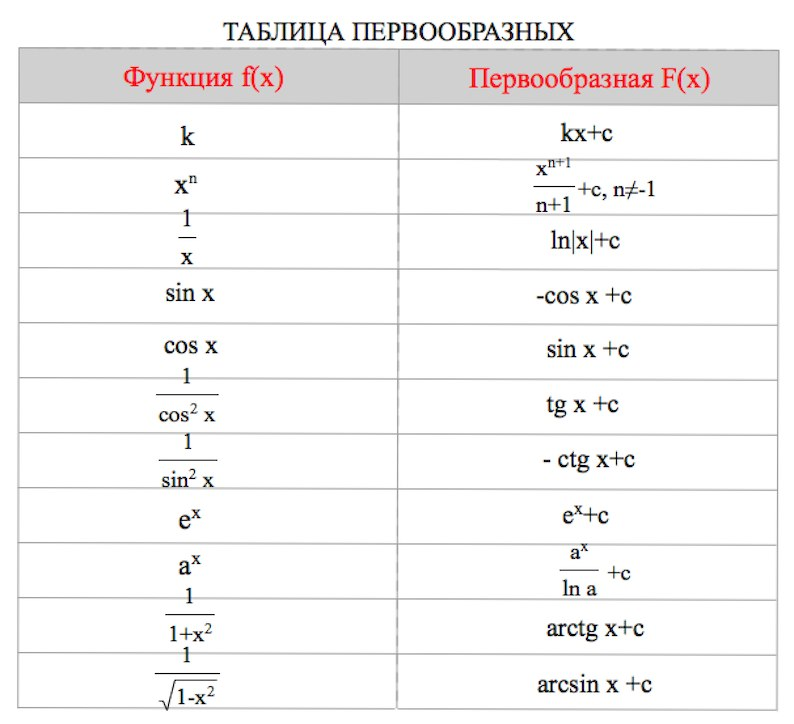
\includegraphics{pervoobraz}
       \begin{comment}
       $$\int \cfrac{dx}{x} = \begin{cases}
         ln(x)+C_1,  & x>0 \\
         -ln(x)+C_2, & x<0 \\
        \end{cases}$$
       \end{comment}
       $$\int sh(x)dx = ch(x)+C_1, \int ch(x)dx = sh(x)+C_2$$

 \item линейность
       $$ \int (f(x) + g(x))dx = \int f(x)dx + \int g(x)dx$$
       $$ \int \alpha f(x) dx = \alpha \int f(x)dx$$
       \begin{exmp}
        $$ \int (x+1)^2 dx = \int (x^2 + 2x + 1)dx = \cfrac{x^3}{3} + x^2 + x + C $$
       \end{exmp}
       \begin{exmp}
        $$ \int \cfrac{x^2}{1+x^2} dx = \int \cfrac{x^2 + 1 -1}{1+x^2} = \int (1 - \cfrac{1}{1+x^2})dx = x - arctg(X) + C $$
       \end{exmp}
 \item интегрирование по частям
       \begin{comment}
       $$(f(x)g(x))'= f'(x)g(x) + f(x)g'(x)$$
       $$ \int (f'(x)g(x) + f(x)g'(x)) dx = f(x)g(x) + C $$
       $$ \int f(x)g'(x) = f(x)g(x)- \int f'(x)g(x) + C$$
       \end{comment}
       \begin{comment}
       Когда использовать: $ \int x^n f(x) dx, \int \dots ln \dots dx, \int \dots arctg \dots dx $
       \end{comment}
       \begin{exmp}
        $$ \int x sin(x) dx = \int x (-cosx)'dx = x(-cosx) - \int (-cosx)dx =$$
        $$= x(-cosx) + \int cos(x)dx=-xcosx + sinx + C$$
       \end{exmp}
       \begin{exmp}
        $$ \int lnx dx = \int x' ln(x) dx = x ln(x) - \int 1 dx = x ln(x) -x + C$$
       \end{exmp}
 \item Замена переменной
       $$f(\phi(x))'= f'(\phi(x))\phi'(x)$$
       Если $\phi(x)$ - дифференцируемая функция, то $y = \phi(x)$
       $$ \int f(\phi(y))dy = \int f(\phi(x))\phi'(x)dx$$
       \begin{exmp}
        $$ \int \cfrac{x}{x^2+1} dx = \int \cfrac{\cfrac{1}{2}}{x^2+1} 2x dx = \int \cfrac{\cfrac{1}{2}}{x^2+1} (x^2)' dx$$
        Обозначим $y = x^2 + 1$
        $$ y = x^2 + 1  $$
        $$ \int  \cfrac{\cfrac{1}{2}}{y}dy = \cfrac{1}{2}ln(y) + C = \cfrac{1}{2}ln(x^2 + 1) + C$$
       \end{exmp}
 \item "Стыковка"
       $$f:[a,c] \Rightarrow \mathbb{R}, a<b<c$$

       $$ F_1(x) \text{- Первообразна на }[a,b]$$
       $$ F_2(x) \text{- Первообразна на }[b,c]$$
       Тогда:
       $$ \int f(x) dx = \begin{cases}
         F_1(x) + C,               & x\in [a,b] \\
         F_2(x) + F_2(b)-F_1(b)+C, & x\in [b,c] \\
        \end{cases}$$
\end{enumerate}
\subsubsection{Первообразная от рациональной функции}
\begin{definition*}
 Рациональная функция - это отношение двух многочленов
 $$R(x)= \cfrac{P(x)}{Q(x)} \text{Где }P(x), Q(x) \text{ - многочлены}$$
\end{definition*}
\begin{name}
 $deg P$ - степень многочлена $P(x) = a_n x^n + a_{n-1}x^{n-1}+ \dots +$\\ $+ a_1 x + a_0, a_n \ne 0$
\end{name}
\begin{comment}
В комплесных числах $$ P(z) = (z - z_1)(z - z_2) \dots (z - z_n)$$
Где $z_1 \dots z_n $ - корни многочлена
Если коэффициенты вещественные:\\
либо корень вещественный,$z_k \in \mathbb{R}$ \\
либо есть комплесно сопряженные $z_k, \overline{z_k}: (z-z_k)(z-\overline{z_k}) = $\\
$= z^2 - (z_k + \overline{z_k})z + z_k \overline{z_k}$
\end{comment}
\begin{lemma}
 Если $P(x)$ - многочлен над $\mathbb{R}$, то его можно разбить на $P(x)= (x-x_1)^{k_1} (x-x_2)^{k_2} \dots (x-x_m)^{k_m} (x^2+ p_1 x+q_1)^{l_1} \dots (x^2+ p_n x+q_n)^{l_n}$
 Это представление едиственно (с точностью до перестановки множителей)
\end{lemma}
\begin{lemma}[о делении с отсатком]
 Если $P(x), Q(x), deg(P) \geq deg(Q),  Q \ne 0$, тогда $\exists{}!$ многочлены $q(x), r(x), deg(q) = deg(P)-deg(Q),\ deg(r) < deg(Q): P(x)=Q(x)q(x)+r(x)$
\end{lemma}
\begin{lemma}
 Еслм $deg(P), deg(Q)>0,$ и $d(x) = NOD(P(x), Q(x))$, тогда $\exists{u(x), v(x)}: deg(u)<deg(Q), deg(v)<deg(P),\\ d(x) = P(x)u(x) + Q(x)v(x)$
\end{lemma}
\begin{theorem}[о разложении в простые дроби]
 Пусть $P(x), Q(x)$ - многочлены, $0 < deg (P) < deg (Q), NOD(P(x), Q(x)) = 1$ и $P(x)$ как в лемме 5, тогда $$\cfrac{P(x)}{Q(x)} = \sum_{i=1}^{m}{\sum_{j=1}^{k_m}{\cfrac{C_{ij}}{(x-x_j)^j}}} + \sum_{i=1}^{n}{\sum_{j=1}^{l_n}{\cfrac{a_{ij}x+b_{ij}}{(x^2 + p_i x + q_i)^j}}}$$
\end{theorem}
\begin{exmp}
 $$ \cfrac{3x^2 - 13x + 5}{x^3 -5x^2 +8x -4} = \cfrac{P(x)}{Q(x)} = R(x)$$
 \begin{enumerate}
  \item Найти корни знаменателя
        $Q(x)=(x-1)(x-2)^2$
  \item теорема о разложении в простые дроби: $R(x) = \cfrac{A}{x-1}+ \cfrac{B}{x-2} + \cfrac{C}{(x-2)^2}$. Найдем коэффициенты $A, B, C$
        $$ 3x^2 - 13x + 5 = A(x-2)^2 + B(x-1)(x-2) + C(x-1)$$
        $$ A = -5, B = 8, C= -9$$
 \end{enumerate}
 $$ \int \cfrac{3x^2 - 13x + 5}{x^3 -5x^2 +8x -4} dx = \int \cfrac{-5}{x-1} dx + \int \cfrac{8}{x-2} dx + \int \cfrac{-9}{(x-2)^2} dx $$
\end{exmp}
\subsubsection{Первообразные простых дробей}
\begin{comment}
$$\int \cfrac{1}{x-x_i} dx = \{y=x - x_i \} = \int \cfrac{dy}{y}= ln\abs{y}+C = ln\abs{x-x_i} + C$$
$$\int \cfrac{1}{(x-x_i)^k} dx = \cfrac{-1}{(k-1)(x-x_i)^{k-1}} + C $$
$$ \int \cfrac{1}{x^2 + px + q} dx = \text{\{Выделим полный квадрат\}} = \int \cfrac{1}{(x- \cfrac{p}{2})^2 + (\underbrace{q- \cfrac{p^2}{4}}_{>0})} dx = $$
$$ = \int \cfrac{1}{a^2((\cfrac{x+\cfrac{p}{2}}{a})^2 + 1)} dx =\{y =\cfrac{x + \cfrac{p}{2}}{a}\} = \int \cfrac{a}{a^2(y^2+1)} dy =\cfrac{1}{a} \int \cfrac{1}{y^2 +1} dy =$$
$$= \cfrac{1}{a} arctg(\cfrac{x}{x} + \cfrac{p}{2a})+ C$$
$$ \int \cfrac{1}{1+x^2} dx = arctgx + C$$
$$ \int \cfrac{x}{1+x^2} dx =\{ y = x^2\}= \int \cfrac{\cfrac{1}{2}dy}{y + 1}  =\cfrac{1}{2}ln(x^2 + 1) + C$$
$$ \int \cfrac{x}{(1+x)^k} dx = \int \cfrac{\cfrac{1}{2}dy}{(1+y)^k}= -\cfrac{1}{2} \cfrac{1}{(k-1)(1+x^2)^{k-1}} + C$$
$$ I_k(y) = \int \cfrac{1}{(1+y^2)^k} dy = \cfrac{y}{1+y^2}^k - \int y(\cfrac{1}{(1+y^2)^k})' dy= \cfrac{y}{1+y^2}^k - \int \cfrac{y(-k(1+y^2)^{k-1} 2y)}{(1+y^2)^{2k}} dy = $$
$$= \cfrac{y}{1+y^2}^k + 2k \int \cfrac{y^2}{(1+y^2)^{k+1}} dy = \cfrac{y}{1+y^2}^k + 2k \int (\cfrac{y^2+1}{(1+y^2)^{k+1}} - \cfrac{1}{(1+y^2)^{k+1}}) dy = $$
$$ = \cfrac{y}{1+y^2}^k + 2k I_k(y) - 2k I_{k+1}(y)$$
$$ I_k(y) = \int \cfrac{1}{(1+y^2)^k} dy$$
$$ I_1(y) = arctg\ y + C$$
$$ I_{k+1}(y) = \cfrac{1}{2k(1+y^2)^k} + \cfrac{2k-1}{2k} I_{k}(y)$$
\end{comment}
\subsubsection{первообразные сводящиеся к рациональным}
$R$ - рациональная функция
\begin{enumerate}
 \item $R(x,\sqrt[n]{ax+b})$ замена $y = \sqrt[n]{ax+b}$ сводит к рациональной функции
       \begin{comment}
       $$\int R(x, \sqrt[n]{ax+b}) dx = \int R(\cfrac{y^n - b}{a}, y) \cfrac{y^{n-1}}{a}dy$$
       \end{comment}
       \begin{exmp}
        $$ \int \cfrac{\sqrt{2x+2}}{\sqrt{x+1} + x - 5} dx \text{\textcircled{ = }}$$
        $$ y = \sqrt{x=1}, x = y^2 - 1, dx = 2ydy $$
        $$ \text{\textcircled{ = }} \int \cfrac{\sqrt{2} y 2y}{y + y^2 - 6} dy = 2\sqrt{2} \int \cfrac{y^2}{y^2+y-6} dy  = 2\sqrt{2} \int (1- \cfrac{y-6}{y^2+y-6}) dy = \dots$$
       \end{exmp}
 \item $R(x, \sqrt[n]{\cfrac{ax+b}{cx+d}}), ad \ne bc$ замена $y=\sqrt[n]{\cfrac{ax+b}{cx+d}}, x = \cfrac{b - dy^n}{cy^n-a} = z(y)$
       $$ \int R(x, \sqrt[n]{\cfrac{ax+b}{cx+d}}) dx = \int R(z(y), y)\cdot z'(y) dy$$
       \begin{exmp}
        $$ \int \cfrac{\sqrt{x+1} - \sqrt{x-1}}{\sqrt{x+1} + \sqrt{x-1}} dx = \int \cfrac{1 - \sqrt{\cfrac{x-1}{x+1}}}{1 + \sqrt{\cfrac{x-1}{x+1}}} dx$$
       \end{exmp}
 \item $R(sinX, cosX)$ универсальная тригонометрическая замена $y = tg(\cfrac{x}{2})$
       $sinx = 2 sin(x/2)cos(x/2) = 2 tg(x/2) cos^2(x/2) = \cfrac{2 y}{1+y}$\\
       $cosx= \cfrac{1-y}{1+y}$ \\
       $dx = \cfrac{2}{1+y} dy$ \\
       Если $R(-sinX, cosX) = - R(sinX, cosX), t = cosX$\\
       Если $R(sinX, -cosX) = - R(sinX, cosX), t = sinX$\\
       Если $R(-sinX, -cosX) =  R(sinX, cosX), t = tgX$\\
 \item $R(shX, chX)$ по аналогии с пунктом (3) + работает замена $y = e^x$
\end{enumerate}
\subsubsection{План изучения}
\begin{itemize}
 \item Формула замены переменной, формула интегрирования по частям
 \item Интегрирование рациональных функций
       \begin{itemize}
        \item Разложение на простые дроби
        \item Метод Остроградского(*)
       \end{itemize}
 \item Интегрирование тригонометрических функций
       \begin{itemize}
        \item $\int R(sinX; cosX) dx \ \ ,  t=tg(\cfrac{x}{2})$ - универсальная подстановка
        \item Четность/нечетность функции $\rightarrow$ специальная замена
        \item Частные случаи(**)
       \end{itemize}
 \item Интегрирование иррациональных функций
       \begin{itemize}
        \item $\int R(x, \sqrt[m]{\cfrac{ax+b}{cx+d}}) dx$
              $$\int R(x, \sqrt[m]{\cfrac{ax+b}{cx+d}}, \sqrt[n]{\cfrac{ax+b}{cx+d}}, \dots ) dx $$
              $t = \sqrt[N]{\cfrac{ax+b}{cx+d}}, N = NOK(m,n, \dots)$
        \item $\int R(x, \sqrt{ax^2+bx+c}) dx$ - выделение полного квадрата или замена Эйлера(***)
        \item Биноминальный интеграл (****)
       \end{itemize}
\end{itemize}
\begin{comment}
Все методы сводятся к интегрированию рациональных функции
\end{comment}

\subsubsection{Частные случаи интегрирования тригонометрических функций}
\begin{enumerate}
 \item $$\int sin^{2m}(x) cos^{2n}(x) dx \ \ \ \ \textit{используя формулы понижения степени получим} $$ $$  \int \cfrac{1-cos(2x)}{2}^m \cfrac{1+cos(2x)}{2}^n dx $$
 \item $$\int sin^{2m+1}(x) cos^{2n}(x) dx = \int sin^{2m}(x) cos^{2n+1}(x) dx = $$
       $$= - \int sin^{2m}(x) cos^{2n}(x) d \underbrace{cos(x)}_{t} = -\int (1-t^2)^m t^{2n} dt$$
 \item $\int sin(ax)cos(bx) dx = (1) $\\
       $\int sin(ax)sin(bx) dx = (2)$\\
       $\int cos(ax)cos(bx) dx = (3)$\\
       $$(1)=\int \cfrac{1}{2}(sin(a+b)x+sin(a-b)x) dx$$
       $$(2)=\int \cfrac{1}{2}(cos(a-b)x-cos(a+b)x) dx$$
       $$(3)=\int \cfrac{1}{2}(cos(a+b)x+cos(a-b)x) dx$$
\end{enumerate}
\subsubsection{\texorpdfstring{$\int R(x, \sqrt{ax^2+bx+c}) dx$}{(***)} }
$$ax^2 +bx +c = a {\underbrace{(x+\cfrac{b}{2a})}_{u}}^2 + c - \cfrac{b^2}{4a}$$
В зависимости от дискриминанта и знака $a$ сводится к:
\begin{itemize}
 \item $\int R(u; \sqrt{a^2-u^2}) du$
 \item $\int R(u; \sqrt{u^2-a^2}) du$
 \item $\int R(u; \sqrt{a^2+u^2}) du$
\end{itemize}
\begin{center}
 \begin{tabular}{ c c c c }
  \hline
  случай           & подстановка (замена)          & $du$                          & корень                        \\
  \hline
  $\sqrt{a^2-u^2}$ & $\begin{aligned}
    u = asin(t) \\
    u = acos(t) \\
   \end{aligned}$ & $\begin{aligned}
    du = acos(t) dt  \\
    du = -asin(t) dt \\
   \end{aligned}$ & $\begin{aligned}
    acos(t) \\
    asin(t) \\
   \end{aligned}$ \\
  \hline
  $\sqrt{u^2-a^2}$ & $\begin{aligned}
    u = \cfrac{a}{sin(t)} \\
    u = \cfrac{a}{cos(t)} \\
   \end{aligned}$ & $\begin{aligned}
    du = -\cfrac{acos(t)}{sin^2 (t)} dt \\
    du = -\cfrac{asin(t)}{cos^2 (t)} dt \\
   \end{aligned}$ & $\begin{aligned}
    \sqrt{(\cfrac{a}{sin(t)})^2 - a^2}=a\ ctg(t) \\
    \sqrt{(\cfrac{a}{cos(t)})^2 - a^2}=a\ tg(t)  \\
   \end{aligned}$ \\
  \hline
  $\sqrt{u^2+a^2}$ & $\begin{aligned}
    u = \cfrac{a}{tg(t)}  \\
    u = \cfrac{a}{ctg(t)} \\
   \end{aligned}$ & $\begin{aligned}
    du = \cfrac{a}{cos^2 (t)} dt  \\
    du = -\cfrac{a}{sin^2 (t)} dt \\
   \end{aligned}$ & $\begin{aligned}
    \sqrt{(\cfrac{a}{tg(t)})^2 - a^2}=\cfrac{a}{cos(t)}  \\
    \sqrt{(\cfrac{a}{ctg(t)})^2 - a^2}=\cfrac{a}{sin(t)} \\
   \end{aligned}$ \\
  \hline
 \end{tabular}
\end{center}
\begin{exmp}
 $$ \int \cfrac{x^2-x+1}{(x^2+1)\sqrt{x^2+1}} dx= \left\{\!\begin{aligned}
   x = tg(t)                  \\
   dx = \cfrac{dt}{cos^2 (t)} \\
   x^2+1 = \cfrac{1}{cos^2 (t)}
  \end{aligned} \right\} = \int \cfrac{tg^2 (t) - tg (t) + 1}{\cfrac{1}{cos^2 (t)}\cdot \cfrac{1}{cos(t)}} \cdot \cfrac{dt}{cos^2 (t)} =$$
 $$ = \int (tg^2(t)+1)cos(t)\ dt - \int tg(t)cos(t)\ dt= \int \cfrac{1}{cos^2t}cos(t)\ dt - \int tg(t)cos(t)\ dt = $$
 $$=\left\{\!\begin{aligned}
   u = tg(\cfrac{t}{2})    \\
   dt = \cfrac{2du}{1+u^2} \\
   cos(t) = \cfrac{2u}{1+u^2}
  \end{aligned} \right\} = \int \cfrac{1+u^2}{2u} \cfrac{2du}{1+u^2} du + cos(t) = ln\abs{u}+cos(t) + C=$$
 $$=ln\abs{tg(\cfrac{arctg(x)}{2})} + cos(arctg(x)) + C$$
\end{exmp}
\subsubsection{Подстановка Эйлера}
$$ \int R(x, \sqrt{ax^2+bx+c}) dx $$
\begin{enumerate}
 \item $a>0\ \ \underbrace{\sqrt{ax^2+bx+c}}_{\text{Корней нет}}=t \pm \sqrt{a}x$
       $$ ax^2 + bx+ c = t^2 \pm 2\sqrt{a}x + ax^2$$
       $$ x = \cfrac{t^2-c}{b \mp 2t \sqrt{a}} \Rightarrow \sqrt{ax^2+bx+c}=t \pm \cfrac{\sqrt{a}(t^2-c)}{b\mp2t \sqrt{a}}$$
       Получаем рациональную функцию под интегралом
 \item 2 различных корня $ax^2+bx+c=a(x-x_0)(x-x_1)$
       $$ t = \cfrac{ \sqrt{ax^2+bx+c}}{x-x_0},\ t^2 (x-x_0)^2 = ax^2+bx+c$$
       $$ t^2(x-x_0) = a(x-x_1)$$
       $$ x = \cfrac{-ax_1 + t^2 x_0}{t^2 - a} \Rightarrow \sqrt{ax^2+bx+c} = t(x-x_0)=$$
       $$ = t(\cfrac{-ax_1 + t^2 x_0}{t^2 - a} - x_0)$$
\end{enumerate}
\subsubsection{Биноминальные интегралы}
$$ \int x^m (ax^n + b)^p dx\ , m,n,p \in \mathbb{Q}$$
\begin{enumerate}[label=\alph*)]
 \item $p$ - целое, тогда по биному Ньютона
 \item $p$ - дробное\\
       Выполнить замену $z=x^n$, тогда $x=z^{\cfrac{1}{n}}, dx=\cfrac{1}{n}z^{\cfrac{1}{n}-1}dz$
       $$ \Rightarrow \int z^{\cfrac{m}{n}}(az+b)^p \cfrac{1}{n}z^{n(\cfrac{1}{n}-1)} dz  =$$
       Вариант 1
       $$= \cfrac{1}{n} \int z^{\cfrac{m+1}{n}-1}(az+b)^p dz\text{, если }\cfrac{m+1}{n} \text{- целое, то}$$
       $$p = \cfrac{\mu}{\nu} \Rightarrow t^{\nu}=az+b=ax^n+b \Rightarrow \text{получим рациональную функцию}$$
       Вариант 2
       $$= \cfrac{1}{n} \int z^{\cfrac{m+1}{n}-1+p}(\cfrac{az+b}{z})^p dz$$
       Если $\cfrac{m+1}{n}+p-1$ - целое, то $t^\nu = \cfrac{az+b}{z}=\cfrac{ax^n+b}{x^n}$
\end{enumerate}
\begin{theorem}[Чебышева]
 $$\int x^m(ax^n+b)^p dx$$ вычесляется в элементарных функциях только, если
 \begin{enumerate}
  \item p-целое
  \item p-дробное, $\cfrac{\mu}{\nu}$ $\left[
         \begin{gathered}
          \cfrac{m+1}{n} \text{ - целое}\hfill,   t^\nu = ax^n+b             \\
          \cfrac{m+1}{n}+p \text{ - целое}\hfill,  t^\nu = \cfrac{ax^n+b}{x^n}
         \end{gathered}
         \right.$
 \end{enumerate}
\end{theorem}
\section{Определенные интегралы}
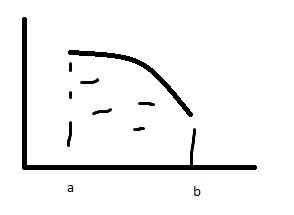
\includegraphics{opr_int}
$$ f:[a,b] \rightarrow R, f(x) \geq 0$$
\begin{formula}[Ньютона-Лейбница]
 $$S = F(b)-F(a) =  \int_a^b f(x) dx, \text{ где } F \text{ - первообразная f}$$
 $$S'(x) = \lim_{\Delta x \rightarrow 0}{\cfrac{S(x +\Delta x)-S(x)}{\Delta x}} = f(x) $$
\end{formula}
\begin{definition*}
 Кольцо множеств - набор множеств замкнутый относительно
 $\cup, \cap, \setminus , \Delta  $
\end{definition*}
\begin{exmp}
 Подмножество $\mathbb{R}^2: $
 \begin{itemize}
  \item Все подмножества пл-ти $P(\mathbb{R}^2)$
  \item $\{\mathbb{R}^2, \emptyset\}$
  \item Все ограниченые множества
  \item Все многоугольники (+$\emptyset$)
 \end{itemize}
\end{exmp}
\begin{definition*}
 Площадь на кольце $R$ подмножеств $\mathbb{R}^2$ это функция $S: R \rightarrow \mathbb{R}$, такая что:
 \begin{enumerate}
  \item $\forall{A} \subset R, S(A) \geq 0$
  \item $ \forall{A,B} \subset R, A\cap B = \emptyset \rightarrow S(A\cup B) = S(A) + S(B)$
  \item не меняется при сдвигах, поворотах, отражениях. Т.е $L:\mathbb{R}^2 \rightarrow \mathbb{R}^2 \Rightarrow S(L(A)) = S(A)$
  \item $S([0,1]^2) = 1$
 \end{enumerate}
\end{definition*}
\begin{comment}
Аналогично $V: R(\mathbb{R}^3) \rightarrow \mathbb{R} $ - объем
\end{comment}
\begin{comment}
Аналогично $l: R(\mathbb{R}) \rightarrow \mathbb{R} $ - длина
\end{comment}
\begin{comment}
\begin{enumerate}
 \item Из определения $S(\subset) = 0$ \\
       $S(A \cup \emptyset) = S(\emptyset) +  S(A)$
 \item $S([0,a] \times [0,b]) = ab$
\end{enumerate}
\end{comment}
\comment Площадь однозначно определяется на кольце многоугольников
\begin{consequence}
 $A \subset B \Rightarrow S(A) \leq S(B) $
\end{consequence}
\begin{proof}
 $$ B = A \cup (B \setminus A) $$
\end{proof}
\begin{definition*}
 Пусть $A\subset \mathbb{R}^2$ - ограниченное множество. \\
 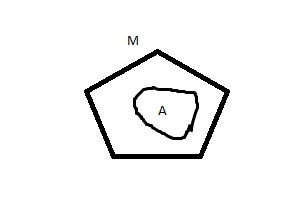
\includegraphics{ploshad}
 $$ S^*(A) = inf(S(M), \text{M - многоугольник}, A\subset M ) \text{ - Внешняя площадь}$$
 $$ S_*(A) = sup(S(M), \text{M - многоугольник}, M \subset A )) \text{ - Внутренняя площадь}$$
 Причем $S^*(A) \geq S_*(A)$
\end{definition*}
\begin{exmp}
 Когда не совпадают:\\
 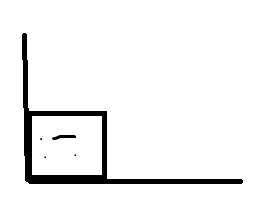
\includegraphics{edinsquare}\\
 $ E = (Q \cap [0,1]^2)$ - точки единичного квадрата с рациональными координатами $\Rightarrow$
 $$  S^*(E) = 1 $$
 $$  S_*(E) = 0 $$
\end{exmp}
\begin{definition*}
 Если $S_*(A) = S^*(A)$, тогда $A$ - квадрируемое
\end{definition*}
\begin{theorem}
 Множество квадрируемых множеств это кольцо. И площадь продолжается на них с сохранением всех свойств
\end{theorem}
\subsubsection{Модель интеграла Дарбу}
\begin{definition*}
 Разбиение отрезка $[a,b]$, это коннечный набор точек $P = \{ a= x_0 <x_1 < x_2< \dots < x_n = b \}$
\end{definition*}
\begin{property*}
 $P_2$ - \textit{подразбиение} $P_1$, если $P_1 \subset P_2$
\end{property*}
\begin{property*}
 У любых двух разбиений есть общее подразбиение
\end{property*}
\begin{definition*}
 Пусть $f: [a,b] \rightarrow \mathbb{R}$ - ограниченая функция.
 Определим \textit{верхний интеграл Дарбу}.\\
 Пусть $P = \{ a= x_0 <x_1 < x_2< \dots < x_n = b \}$. На каждом отрезке $A_i = [x_i;x_{i+1}]$ выберем $C_i \geq f(x) \forall{x} \in A$.
 $$ \int_a^{b*} f(x)  dx = inf_{P, C_i}\{\sum_{i=0}^{n-1}{C_i(x_{i+1}-x_i)}\} $$
 Аналогично определяется \textit{нижний интегралл Дарбу}
 $$ \int_{a*}^{b} f(x)  dx = $$
 $$=sup_{P, C_i}\{\sum_{i=0}^{n-1}{C_i(x_{i+1}-x_i), P = \{ a= x_0 <x_1 < x_2< \dots < x_n = b \}, C_i \leq f(x) \forall{x} \in [x_i;x_{i+1}]\}} $$
\end{definition*}
\begin{comment}
$$ \int_{a*}^{b} f(x)  dx \leq \int_a^{b*} f(x)  dx$$
\end{comment}
\begin{exmp}
 $$f_D: [0,1] \rightarrow [0,1]$$
 $$ f_D(x) = \begin{cases}
   1, & x\in \mathbb{Q}     \\
   0, & x \notin \mathbb{Q} \\
  \end{cases}$$
\end{exmp}
\begin{comment}
Если они совпадают, то $f$ \textit{интегрируема по Дарбу}
$$\int_a^b f(x)  dx = \int_{a*}^{b} f(x)  dx = \int_a^{b*} f(x)  dx$$
Интеграл Дарбу функции $f$ на отрезке $[a,b]$
\end{comment}
\subsubsection{Модель интегралла Римана}
$$\text{Пусть } f:[a,b] \rightarrow \mathbb{R}$$
$ \tau = \{ a= x_0 <x_1 < x_2< \dots < x_n = b \} $\\
Набор точек $\{ \xi_1, \dots ,\xi_n \}$ - подчиненён разбиению P, если $$ \xi_i\in[x_{i-1}m x_i] $$
\begin{formula}[Сумма Римона]
 $$ S(f, P, \xi)=\sum_{i=1}^{n}{f(\xi_i)(x_i-x_{i-1})} $$
\end{formula}
\begin{definition*}
 \textit{Шаг разбиения}: $\Delta(\tau) = max_{i=1, \dots,n} (x_i - x_{i-1})$
\end{definition*}
\begin{definition*}
 \textit{Интеграл Римона}
 $I$ - называется интегралом Римона, если $f$ на $[a,b]$,если
 $$ \forall{\varepsilon}>0 \exists{\delta}>0: \abs{I-S(f, \tau, \xi)}<\varepsilon $$
 $$ \int_a^b f(x)  dx = \lim_{\Delta(P) \rightarrow 0}{S(f,\tau,\xi)} $$
 Если этот предел существует и независит от $\tau, \xi$
\end{definition*}
\begin{exmp}
 $f \equiv c $ на [a,b]
 $$ S(f, \tau, \xi) = c(b-a) $$
\end{exmp}
\begin{exmp}
 $$D(X) = \begin{cases}
   1, & \text{рац на }[0,1] \\
   0, & \text{ир на }[0,1]  \\
  \end{cases}$$
 $\forall{\tau} $ - разбиение $[0,1]$ $\exists{\xi_k` }\in \mathbb{Q}, \xi_k``  \notin \mathbb{Q} $
 $$S(D, \tau, \xi_k`  ) = \sum_{n=1}^{\infty}{1(x_k - x_{k-1})} = 1$$
 $$S(D, \tau, \xi_k`` ) = \sum_{n=1}^{\infty}{0(x_k - x_{k-1})} = 0 $$
 $$ \InAll \nexists lim $$
\end{exmp}
\begin{exmp}
 $$R(X) = \begin{cases}
   \cfrac{1}{n}, & x = \cfrac{m}{n} \text{несократима} \\
   0,            & x \notin \mathbb{Q}                 \\
  \end{cases} \text{ на [a,b]}$$
 $$ S(R, \tau, \xi) = \sum_{i=0}^{k}{R(\xi_i)\delta x_i} = \sum_{R(\xi_i) < \cfrac{1}{N}}{R(\xi_i)\delta x_i}+ \sum_{R(\xi_i) \geq \cfrac{1}{N}}{R(\xi_i)\delta x_i} <$$
 $$ < \sum_{R(\xi_i) < \cfrac{1}{N}}{\cfrac{1}{N} \delta x_i} + \sum_{R(\xi_i) \geq \cfrac{1}{N}} {1 \delta x_i} < \cfrac{1}{N} \sum_{R(\xi_i) < \cfrac{1}{N}}{\delta x_i} + \Delta (\tau) \text{кол-во } \{R(\xi_i) \geq \cfrac{1}{N} \} <$$
 Грубой оценкой является $N^2$\\
 $N = 1, x = 1  \longrightarrow1$\\
 $N = 2, x = 1, x = \cfrac{1}{2} \longrightarrow2$\\
 $N = 3, x = 1, x = \cfrac{1}{2}, x = \cfrac{1}{3}, x = \cfrac{2}{3} \longrightarrow 4$\\
 Далее, если кол-во $\{x: R(x) \geq \cfrac{1}{N} \}$ не более $N^2$, то для $\funcSet{x}{R(x) \geq \cfrac{1}{N+1}}$ могут добавляться дроби $\cfrac{k}{N+1}$, $k = 1, \dots, n$\\
 Т.е добавится не более $N$ штук $N^2+N <(N+1)^2$
 $$S(R, \tau, \xi) < \cfrac{1}{N}+\Delta(\tau)N^2$$
 Засчет выбора достаточно малого $\Delta(\tau): \forall{\varepsilon}>0\ \exists{N}\ \ \cfrac{1}{N}<\cfrac{\varepsilon}{2} $ и $\Delta = \cfrac{1}{N^3}$\\
 $\Rightarrow \forall{\tau}: \Delta(\tau) < \delta $ получаем:
 $$\abs{0 - S(R, \tau, \xi)} = \cfrac{1}{N} +\delta N^2 = \cfrac{1}{N} + \cfrac{N^2}{N^3}=\cfrac{2}{N} < 2 \cfrac{\varepsilon}{2} = \varepsilon \Rightarrow \int\limits_0^1 R(x)  dx $$
\end{exmp}
\subsubsection{Верхние и нижние суммы Дарбу}
\begin{definition*}
 Пусть $f: [a,b] \rightarrow \mathbb{R}$ - ограниченая функция.
 Определим \textit{верхняя сумма Дарбу}.\\
 $f$ - огр на $[a,b]$
 $$ M_k = \sup_{[x_k, x_{k-1}]}(f(x)), m_k = \inf_{[x_{k-1}, x_k]}(f(x)) $$
 $$S_\tau = \sum_{k=0}^{n}{M_k \Delta x_k} , s_\tau = \sum_{k=0}^{n}{m_k \Delta x_k}$$
\end{definition*}

\begin{property}
 $$ s_\tau \leq S(f, \tau, \xi) \leq S_\tau \  \forall{\xi}$$
\end{property}
\begin{property}
 $$ \tau' \subseteq \tau'' \Rightarrow S_{\tau''} \leq S_{\tau'}$$
\end{property}
\begin{property}
 $$\forall{\tau', \tau''}: s_{\tau'} \leq S_{\tau''} $$
 Нижний предел:
 $$ \sup_{\tau} (s_\tau) = \underline{I} = \int\limits_{a*}^b f(x)dx$$
 Верхний предел:
 $$ \inf_{\tau} (S_\tau) = \overline{I} = \int\limits_{a}^{b*} f(x)dx$$
\end{property}
\begin{property}
 $$\forall{\varepsilon}>0\ \exists{\tau}\ \exists{\overline{\xi}}: 0 \leq S_\tau - S(f,\tau, \overline{\xi})< \varepsilon $$
\end{property}
\begin{proof}
 По определению $M_k \exists{\xi_k} \in [x_{k-1}, x_k]: M_k - f(\xi_k) < \cfrac{\varepsilon}{b-a}, \underline{\xi} ={\xi_k}$
 $$S_\tau - S(f, \tau, \underline{\xi}) = \sum_{i=0}^{n}{(M_k-f(\xi_k)) \Delta x_k} < \cfrac{\varepsilon}{b-a}\sum_{i=0}^{n}{\Delta x_k} = \varepsilon$$
\end{proof}
\begin{property}
 $$\forall{\varepsilon}>0\ \exists{\tau}\ \exists{\underline{\xi}}: 0 \leq  S(f,\tau, \underline{\xi}) - S_\tau < \varepsilon $$
\end{property}
\begin{property}
 Пусть $\tau'$ полученна из $\tau$ путем добавления $p$ точек. Тогда $S_\tau - S_{\tau'} \leq (M-m)p\Delta(\tau)$ , $S_{\tau'} - S_{\tau} \leq (M-m)p\Delta(\tau)$
\end{property}
\begin{proof}
 добавление 1 точки: $x_{k-1} < x' < x_k$
 $$S_\tau - S_{\tau'} = M_k(x_k - x_{k-1}) - (M_k'(x_k - x') + M_k''(x'-x_{k-1}))= $$
 $$= (M_k-M_{k'})(x_k-x') + (M_k - M_{k}'')(x'-x_{k-1}) \leq (M-m)\Delta(\tau)$$
 Далее по индукции\\
\end{proof}
\begin{lemma}[Дарбу]
 $$\overline{I} = \lim_{\Delta(\tau) \rightarrow 0}{S_\tau}$$
 $$\underline{I} = \lim_{\Delta(\tau) \rightarrow 0}{s_\tau}$$
\end{lemma}
\begin{proof}
 $M=m \Rightarrow f(x) = const = m = M\ \underline{I} = s_\tau, \overline{I}=S_\tau$
 $$ M > m, \forall{\varepsilon}\ \exists{\tau^*}: S_{\tau^*}-\underline{I}<\cfrac{\varepsilon}{2} \text{по опр inf} $$
 Пусть $p$ - кол-во точек $\tau^*$, лежащие внутри $[a,b]$. Выберем $$\delta = \cfrac{\varepsilon}{2(M-m)p}$$
 Пусть $\tau : \Delta(\tau) < \delta, $ $\tau' = \tau \cup \tau^*$ \\
 $$ S_\tau - \underline{I} = S_\tau - S_{\tau'} + S_{\tau'} - \underline{I} \leq (M-m)p\Delta(\tau) + S_{\tau'} - \underline{I} < \cfrac{\varepsilon}{2} + \cfrac{\varepsilon}{2} = \varepsilon $$
 Для второго \textit{УПР!}
\end{proof}
\begin{theorem}[Критерий Дарбу интегрируемости по Римону]\label{th:krDarbu}
 Ограниченная на $[a,b]$ ф-ция $f$ интегрируема по Римону $\Leftrightarrow \ \forall{\varepsilon}>0\ \exists{\tau}:\ S_\tau - s_\tau < \varepsilon$
\end{theorem}
\begin{proof}
 $\Rightarrow$\\
 Тогда $\exists{\delta}> 0 $ из определения инт-мости выберем $\tau: \Delta(\tau)< \delta \  $
 $$ \abs{I - S(f, \tau, \xi)} <\cfrac{\varepsilon}{4}\ \forall{\xi} $$
 По св-ву 4 и 5 выберем $\underline{\xi}, \overline{\xi}$:
 $$ S_\tau - S(f,\tau, \overline{\xi}) < \cfrac{\varepsilon}{4}, \ S(f, \tau, \underline{\xi})- s_\tau<\cfrac{\varepsilon}{4} $$
 $$S_\tau-s_\tau = S_\tau - S(f, \tau, \overline{\xi}) + S(f,\tau, \overline{\xi})- I + I - S(f,\tau, \underline{\xi}) +S(f,\tau, \underline{\xi}) -s_\tau < \varepsilon  $$
 $ \Leftarrow $\\
 Из условия следует: $\underline{I} = \overline{I} = I$ - обозначение. \\
 По лемме Дарбу: по $\varepsilon $ выберем $\delta: \Delta(\tau) < \delta$\\
 $$S_\tau - I < \cfrac{\varepsilon}{2}, I- s_\tau < \cfrac{\varepsilon}{2} \Rightarrow $$
 $$ \Rightarrow \forall{\xi} \text{ по св-ву 1} \abs{S(f,\tau,\xi) -I}<\varepsilon $$
\end{proof}
\begin{memories}
 В прошлом семестре вводилось определение колебания функции $f$ на $[x_{k-1}, x_k]$:
 $$ \omega_k = \sup_{x',x'' \in [x_{k-1}, x_k]} \abs{f(x'')-f(x')} $$
\end{memories}
Очевидно, что
$$ \omega_k = \underbrace{M_k}_{\sup_{[x_{k-1}, x_k]} f(x)} + \underbrace{m_k}_{\inf_{[x_{k-1}, x_k]} f(x)} $$
Следовательно,
$$ \underbrace{S_\tau - s_\tau}_{\text{Эта разность фигурирует в Теореме 1}} = \sum_{k=1}^{n}{\omega_k \Delta x_k} $$
\begin{consequence*}
 Ограниченная на $[a,b]$ функция $f$ интегрируема\\ $\Leftrightarrow \forall{\varepsilon} > 0 \ \exists{\text{ Разбиение }\tau}: \sum_{k=1}^{m}{\omega_k \Delta x_k} < \varepsilon$
\end{consequence*}
\subsection{Некоторые классы интегрируемых функций}
\subsubsection{Некоторые классы интегрируемых функций}
\begin{theorem}[Основное св-во интегрируемых функций, необходиоме условие]
 Если функция $f$ интегрируема на $[a,b]$, то она ограничена на $[a,b]$
\end{theorem}
\begin{proof}[От противного]
 Пусть $f$ не ограничена на $[a,b]$ и пусть выбрано разбиение $\tau: a = x_0<x_1< \dots < x_k = b$\\
 Т.к $f$ не ограничена на $[a,b]$, то $f$ не ограничена на каком-то маленьком отрезке разбиения. Пусть это будет $[x_0, x_1]$. Тогда $\exists{}$ последовательность $\xi_1^{(n)} \in [x_0,x_1]\text{(здесь (n) просто номер $\xi_1$ )}, n=1,2, \dots$, такая, что $\lim_{n \rightarrow \infty}{f(\xi_1^{(n)})} = \infty$\\
 Фиксируем точки на других отрезках: $\xi_i\in[x_{i-1}, x_{i}]$. Тогда для данного $\tau$ и $\xi_i$ сумма $\sum_{i =2}^{k}{f(\xi_i)\Delta x_i}$  какое-то определенное число.\\
 $$ \InAll \lim_{n \rightarrow \infty}{S(f,\tau,\xi)} = \lim_{n \rightarrow \infty}{S(f,\tau, \xi_1^{(n)}, \xi_2, \xi_3, \dots )} = $$
 $$= \lim_{n \rightarrow \infty}{( \underbrace{f(\xi_1^{(n)})}_{\rightarrow \infty}\Delta x_1 + \underbrace{\sum_{i =2}^{k}{f(\xi_i)\Delta x_i} }_{\text{Число}})} = \infty$$
 \begin{equation}
  \InAll \forall{M} > 0\ \exists{n_0}: \abs{S(f,\tau, \xi_1^{n_0}, \xi_2, \xi_3, \dots, \xi_k ) }>M \label{eq:ref}
 \end{equation}
 $\InAll $ интегральные суммы не могут стремиться к конечному пределу при $\Delta(\tau) \rightarrow 0$\\
 Действительно, если $\exists{\lim_{\Delta(\tau) \rightarrow 0}{S(f,\tau, \xi)}} = A$ - конечное, то
 $$\forall{\varepsilon}>0 \ \exists{\delta}: \forall{\tau}: \Delta (\tau) < \delta\ \forall{\xi}\ \abs{S(f, \tau, \xi) - A} <\varepsilon $$
 $$\InAll \abs{S(f,\tau, \xi)} \leq \abs{S(f,\tau, \xi) - A} + \abs{A} < \varepsilon + \abs{A} $$
 А мы получили в \ref{eq:ref}, что $\forall$разбиения $\tau$ при фиксированном $\varepsilon$ можно выбрать $\xi$ так, что $\abs{S(f,\tau, \xi)}>\abs{A} + \varepsilon= M \Rightarrow \bot$\\
\end{proof}
\begin{theorem}
 Непревная на отрезке функция - интегрируема
\end{theorem}
\begin{proof}
 По теореме Кантор, любая непрерывная на отрезке функция - равномерно непрерывна:
 $$ \forall{\varepsilon}>0\ \exists{\delta}: \abs{x'-x''}<\delta \Rightarrow \abs{f(x') - f(x'')} < \varepsilon $$
 Рассмотрим разбиение $\tau$ такое, что $\Delta(\tau) < \delta$, тогда если $x', x''\in [x_{k-1};x_k], то \abs{f(x') -f(x'')}<\varepsilon$
 $$ \sup_{x', x''}{\abs{f(x')-f(x'')}} = \sup{(f(x'))} - \inf{(f(x''))} = M_k - m_k \leq \varepsilon \text{ Равенство появилось из-за sup} $$
 $$ \Rightarrow S_\tau - s_\tau = \sum{M_k-m_k}\Delta x_k \leq \varepsilon(b-a) $$
 $  \Rightarrow $ по критерию Дарбу (\ref{th:krDarbu}) функция интегрируема\\
\end{proof}
\begin{theorem}
 Если $f$ имеет конечное число разрывов и ограничена на $[a,b]$, то $f$ интегрируема
\end{theorem}
Эта теорема будет следовать из более сильной теоремы
\begin{theorem*}[3!]\label{th:Sec_3_pr_1_3!}
 Пусть $f$ ограничена на $[a,b]$ и для любого $\varepsilon > 0$ можно указать конечное число интервалов, покрывающих все точки разрыва $f$ и имеющих общую сумму длин меньшую, чем $\varepsilon$, то $f$ интегрируема на $[a,b]$
\end{theorem*}
\begin{proof}
 $\varepsilon > 0$. Покроем все разрывы конечным числом интервалов общей длинны меньше чем $\cfrac{\varepsilon}{2(M-m)}$
 \\
 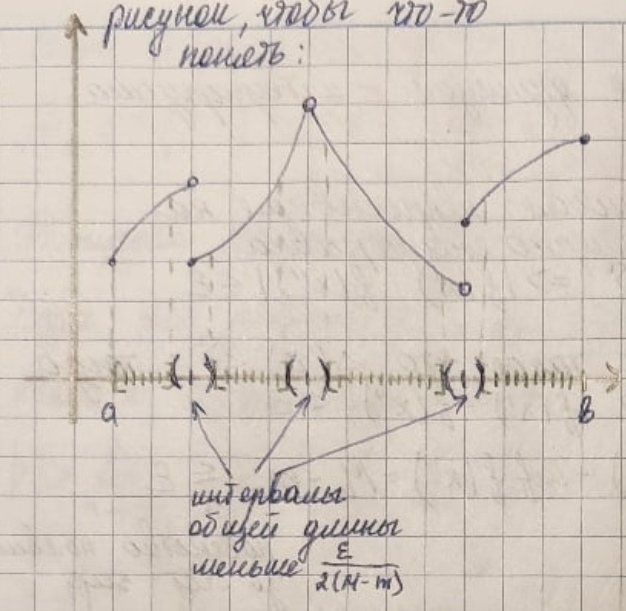
\includegraphics[scale = 0.5]{1903202020pic}\\
 Если из $[a,b]$ удалить конечное число интервалов, то останется объединение конечного числа отрезков на которых $f$ непрерывна.\\
 Разобъем каждый отрезок так, что колебание $\omega_i$ там меньше, чем $\cfrac{\varepsilon}{2(M-m)}$\\
 Объеденим эти разбиения и интервалы с разрывами получаем некоторое разбиение $\tau$\\
 Итак,
 $$ S_\tau - s_\tau = \sum{\omega_k \Delta x_k} = \underbrace{\sum {\omega_i \Delta x_i }}_{\text{Сумма по всем маленьким отрезкам}} + \underbrace{\sum {\omega_j \Delta x_j }}_{\text{Сумма по всем интервалам}} < $$
 $$< \cfrac{\varepsilon}{2(b-a)} \cdot \underbrace{\sum{\Delta x_i}}_{\substack{\text{по маленьким отрезкам,} \\ \text{длинны в сумме}\\ <(b-a)}} + \underbrace{(M-m)\sum{\Delta x_j}}_{\substack{\text{по интервалам,}\\ \text{их длинна} < \cfrac{\varepsilon}{2(M-m)}}} < \cfrac{\varepsilon}{2} + \cfrac{\varepsilon}{2} = \varepsilon $$
 $\InAll$ по критерию  Дарбу \ref{th:krDarbu} функция интегрируема\\
\end{proof}
\begin{comment}
В теореме 3' \ref{th:Sec_3_pr_1_3!} и на рисунке точек разрыва может быть бесконечно числом
\end{comment}
\begin{theorem}[Критерий Лебега]
 Пусть $f$ огграничена на $[a,b]$. $f$ интегрируема $\Leftrightarrow$ множество точек разрыва обладает свойством: $\forall{\varepsilon}>0\ \exists{I_n}$ - конечная или бесконечная посл-ть интервалов такая, что \\
 $\Set{\text{множество точек разрыва}} \subset \bigcup I_n$ и $\sum_{n=1}^{\infty}{\abs{I_n}<\varepsilon}$ (другими словами, мн-во точек разрыва меры 0\label{def:mera_0})
\end{theorem}
\begin{theorem}
 Монотонная на $[a,b]$ функциия - интегрируема
\end{theorem}
\begin{proof}
 $f - \underbrace{\text{монотонная}}_{\text{(пусть возврастает)}} \Rightarrow f(a) \leq f(x) \leq f(b)\ \forall{x} \in [a,b]$\\
 Пусть $\varepsilon>0$. $\tau$ - разбиение $[a,b]$ на равные отрезки длинной меньше $\cfrac{\varepsilon}{f(b)-f(a)}$, т.е $\Delta(\tau) < \cfrac{\varepsilon}{f(b)-f(a)}$ \\
 Очевидно, что $\forall{[x_{i-1}, x_i]}\ m_i = f(x_{i-1}), M_i = f(x_i)$, т.к $f$ возврастает $\Rightarrow S_\tau - s_\tau = \sum{(M_i-m_i)\Delta x_i}= \sum{(f(x_i)-f(x_{i-1}))} \leq \Delta(\tau) \sum{(f(x_i)-f(x_{i-1}))} = $
 $$ = \Delta(\tau)(f(b)-f(a)) <\varepsilon $$
 $\InAll$ по критерию Дарбу \ref{th:krDarbu} функция интегрируема
\end{proof}
\subsection{Пространство интегрируемых функций. Основные свойства интеграла}
$\mathcal R_{[a,b]}$ - множество интегрируемых функций на отрезке $[a,b]$\\
Мы уже выяснили, что в этом мн-ве лежат непрерывные, монотонные, разрывные функции с мн-вом разрывных точек разрыва меры 0 (\ref{def:mera_0})
\begin{theorem}
 Пусть $f, g \in \mathcal R_{[a,b]} $, тогда:
 \begin{enumerate}
  \item $f+g \in \mathcal R_{[a,b]}$
  \item $df \in \mathcal R_{[a,b]}$
  \item $\abs{f} \in \mathcal R_{[a,b]}$
  \item $fg \in \mathcal R_{[a,b]}$
  \item Пусть $[c,d]\subset[a,b]$. Тогда если $f \in \mathcal R_{[a,b]}, то f \Biggr|_{[c,d]} \in \mathcal R_{[a,b]}$
 \end{enumerate}
\end{theorem}
\begin{proof}
 \begin{enumerate}
  \item Пусть $\tau$ - разбиение $[a,b], \Set{\xi_i} = \xi $ - отмечены.\\
        Тогда $S(f+g, \tau, \xi) = \sum_{i=1}^{k}{(f(\xi_i)+g(\xi_i))\Delta x_i} = S(f,\tau, \xi) + S(g, \tau, \xi)$\\
        T.k $\exists{\lim_{\Delta(\tau) \rightarrow 0}{S(f, \tau, \xi)}} и \exists{\lim_{\Delta(\tau) \rightarrow 0}{S(п, \tau, \xi)}}$, то $\exists{\lim_{\Delta(\tau) \rightarrow 0}{S(f+g, \tau, \xi)}}$ \\

        $\InAll f+g \in \mathcal R_{[a,b]}$ и $\int\limits_{a}^{b} (f+g)  dx = \int\limits_{a }^{b } f dx + \int\limits_{a }^{b } g dx$
  \item Аналогично 1)
  \item Аналогично 1)
  \item Удобнее на языке колебаний \\
        $f,g \in \mathcal R_{[a,b]} \Rightarrow $ они ограничены $\Rightarrow \exists{A}> 0, B>0:$
        $$ \abs{f(x)} \leq A, \abs{g(x )} \leq B\ \forall{x} \in [a,b] \Rightarrow \abs{f(x)g(x)} \leq AB\  \forall{x} \in [a,b]$$
        Пусть $\tau$ - разбиение $[a,b]$. Рассмотрим разность из определения колебаний ф-ции fg:
        $$ \abs{f(x'')g(x'') - f(x')g(x')} = \abs{f(x'')g(x'') -f(x')g(x'') + f(x')g(x'') - f(x')g(x')} =$$
        $$=  \underbrace{\abs{f(x'')-f(x')}}_{\substack{\text{Разность из } \\ \text{опр. колебания}\\ \text{функции f}}}\cdot \underbrace{\abs{g(x'')}}_{ \leq B}+ \underbrace{\abs{g(x'')-g(x')}}_{\substack{\text{Разность из } \\ \text{опр. колебания}\\ \text{функции g}}} \cdot \underbrace{\abs{f(x')}}_{ \leq A}$$
        Следовательно, $\forall{x',x''} \in [x_{i-1},x_i]$
        $$ \abs{f(x'')g(x'') - f(x')g(x')} \leq B \omega_i(f) + A \omega_i(g) \Rightarrow \omega_i(fg) \leq B \omega_i(f) + A \omega_i(g) $$
        Получаем:
        \begin{equation}
         \sum_{i=1}^{k}{\omega_i(fg)\Delta x_i} \leq B \sum_{i=1}^{k}{\omega_i(f)\Delta x_i} + A \sum_{i=1}^{k}{\omega_i(g)\Delta x_i}
         \label{eq:ref_2}
        \end{equation}
        %TODO: ЧТО ЗА ТЕОРЕМА 2.2??
        $f$ и $g$ интегрируема $\Rightarrow$ по теореме 2 пр.2 $\forall{\varepsilon} > 0 \ \exists{\tau_{1,2}}: $ (у каждой ф-ции своё)
        $$ \sum_{i=1}^{k}{\omega_i(f) \Delta x_i}<\varepsilon, \sum_{i=1}^{k}{\omega_i(g) \Delta x_i}<\varepsilon $$
        $\InAll$ правая часть неравенства \ref{eq:ref_2} $\rightarrow 0 \Rightarrow $ левая часть неравентсва $\rightarrow 0 \Rightarrow $ по той же тореме 2 пр.2 $fg$ - интегрируема
  \item 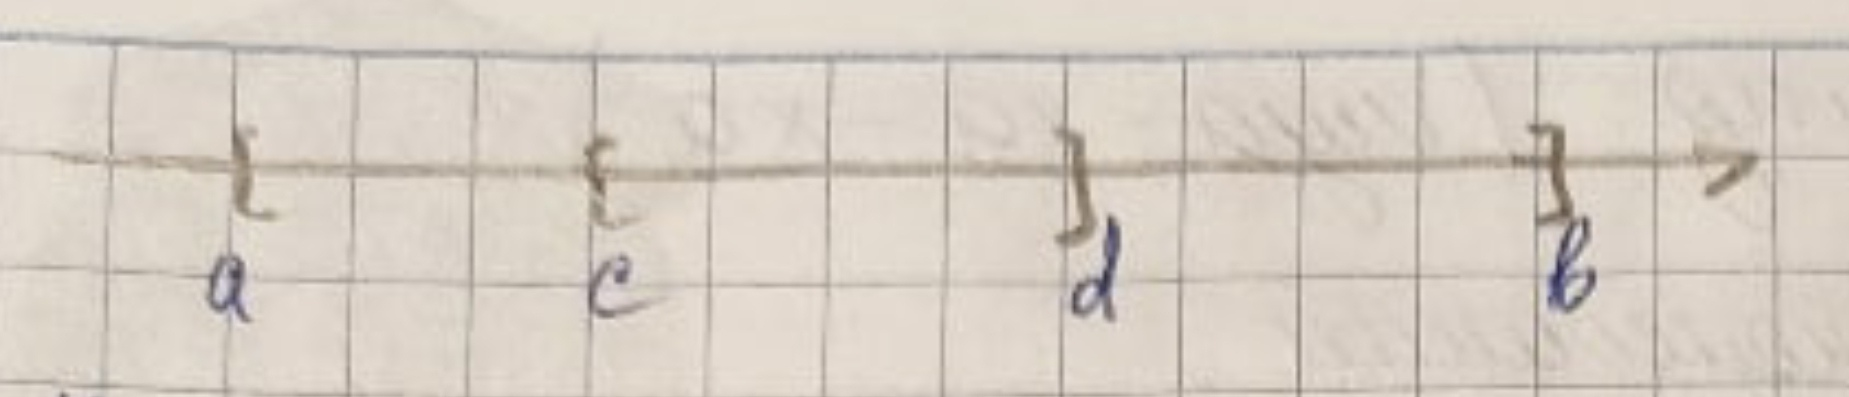
\includegraphics[scale=0.1]{1903202020pic_2}\
        $[c,d] \subset [a,b]$\\
        Простые факты:
        \begin{enumerate}
         \item Если $f$ ограничена на $[a,b]$, то $f$ ограничена на $[c,d]$
         \item Пусть $\tau$ - разбиение $[c,d]$ мелкости $\Delta(\tau)$. Тогда можно добавить к точкам из $\tau$ конченое число точек принадлежащих $[a,b] \setminus [c,d]$, причем в так, чтобы объединение этих точек с $\tau_1$ давало разбиение $\tau$ с мелкостью $\Delta(\tau_1) = \Delta(\tau)$\\
               Получаем:
               $$ 0 \leq S_\tau - s_\tau  = \sum_{\substack{\text{суммирование}\\ \text{по разбиению } \tau}}{(M_i-m_i)\Delta x_i} \leq $$
               $$ \leq \sum_{\substack{\text{суммирование}\\ \text{по разбиению } \tau_1, \\ \text{слагаемых больше}}}{(M_i-m_i)\Delta x_i} = S_{\tau_1} - s_{\tau_1} \xrightarrow[\substack{\text{по кр Дарбу}\ref{th:krDarbu}\\ f \text{ -интегр. на } [a,b]}]{} 0$$
               $\InAll S_\tau - s_\tau \rightarrow 0 \Rightarrow f$ интегрируема на $[c,d]$
        \end{enumerate}
 \end{enumerate}
\end{proof}
\end{document}
